\documentclass[english,nohyper,titlepage]{tufte-handout}\usepackage{knitr}
\usepackage{charter}
\usepackage{helvet}
\renewcommand{\familydefault}{\rmdefault}
\usepackage[latin9]{inputenc}
\usepackage{color}
\usepackage{natbib}
%\usepackage{cite}
\usepackage{babel}
\usepackage{graphicx}
\usepackage{amsmath}
\usepackage[unicode=true,pdfusetitle,bookmarks=true,bookmarksnumbered=false,bookmarksopen=false,
            breaklinks=false,pdfborder={0 0 0},backref=false,colorlinks=true] {hyperref}
\hypersetup{urlcolor= RedOrange, citecolor=RedOrange, linkcolor=RedOrange}
\fancyhf{}% clear previous contents of running heads/feet
\fancyhead[RE]{\footnotesize{Machine Learning\qquad{} \thepage}}
\fancyhead[LO]{\footnotesize{\thepage \qquad{}Applications in R}}
%\rhead{myrhead}
\makeatletter
\newcommand{\sgn}{\operatorname{sgn}} %define the sign operator


\title{\LARGE An Introduction to Machine Learning \\ 
\noindent \normalsize With Applications in R\normalsize}

\author{{\small Michael Clark\\
         \noindent Center for Social Research\\
         \noindent University of Notre Dame\\}}
%% Because html converters don't know tabularnewline
\providecommand{\tabularnewline}{\\}


\AtBeginDocument{
\def\labelitemi{} %%%%\(\cdot\) remove bullet
}

\makeatother
\IfFileExists{upquote.sty}{\usepackage{upquote}}{}

\begin{document}
\bibliographystyle{apa}

\maketitle
\pagebreak{}
\tableofcontents{}
\pagebreak{}



%%%%%%%%%%%%%%%%%%%%%%%%%%%%%%%%%%%%%%
\part{Preface}

The purpose of this document is to provide a conceptual introduction to statistical or machine learning (ML) techniques for those that might not normally be exposed to such approaches during their typical required statistical training\sidenote{I generally have in mind social science researchers but hopefully keep present the material broadly enough for anyone that may be interested.}.  Machine learning\sidenote{Also referred to as applied statistical learning, statistical engineering, data science or data mining in other contexts.} can be described as a form of a statistics, often even utilizing well-known and familiar techniques, that has bit of a different focus than traditional analytical practice in the social sciences and other disciplines.  The key notion is that flexible, automatic approaches are used to detect patterns within the data, with a primary focus on making predictions on future data.

If one surveys the number of techniques available in ML without context, it will surely be overwhelming in terms of the sheer number of those approaches, as well as the various tweaks and variations of them.  However, the specifics of the techniques are not as important as more general concepts that would be applicable in most every ML setting, and indeed, many traditional ones as well.  While there will be examples using the R statistical environment and descriptions of a few specific approaches, the focus here is more on ideas than application\sidenote{Indeed, there is evidence that with large enough samples many techniques converge to similar performance.} and kept at the conceptual level as much as possible.  However, some applied examples of more common techniques will be provided in detail.

As for prerequisite knowledge, I will assume a basic familiarity with regression analyses typically presented to those in applied disciplines, particularly those of the social sciences.  Regarding programming, one should be at least somewhat familiar with using R and Rstudio, and either of my introductions \href{http://www.nd.edu/~mclark19/learn/Introduction_to_R.pdf}{here} and \href{http://www.nd.edu/~mclark19/learn/Introduction_to_R_II.pdf}{here} will be plenty.  Note that I won't do as much explaining of the R code as in those introductions, and in some cases I will be more concerned with getting to a result than clearly detailing the path to it.  Armed with such introductory knowledge as can be found in those documents, if there are parts of R code that are unclear one would have the tools to investigate and discover for themselves the details, which results in more learning anyway.

\marginnote{The latest version of this document is dated \today{} (original March 2013).}
\pagebreak{}


% !Rnw root = ../mlcrash.Rnw




%%%%%%%%%%%%%%%%%%%%%%%%%%%%%%%%%%%%%%%%%%%%%%
\part{Introduction: Explanation \& Prediction}
%%%%%%%%%%%%%%%%%%%%%%%%%%%%%%%%%%%%%%%%%%%%%%
\newthought{For any particular analysis conducted}, emphasis can be placed on understanding the underlying mechanisms which have specific theoretical underpinnings, versus a focus that dwells more on performance and, more to the point, future performance.  These are not mutually exclusive goals in the least, and probably most studies contain a little of both in some form or fashion.  I will refer to the former emphasis as that of \emph{explanation}, and the latter that of \emph{prediction}.

In studies with a more explanatory focus, traditionally analysis concerns a single data set.  For example, one assumes a data generating distribution for the response, and one evaluates the overall fit of a single model to the data at hand, e.g. in terms of R-squared, and statistical significance for the various predictors in the model.  One assesses how well the model lines up with the theory that led to the analysis, and modifies it accordingly, if need be, for future studies to consider.  Some studies may look at  predictions for specific, possibly hypothetical values of the predictors, or examine the particular nature of individual predictors effects.  In many cases, only a single model is considered.  In general though, little attempt is made to explicitly understand how well the model will do with future data, but we hope to have gained greater insight as to the underlying mechanisms guiding the response of interest.  Following \citet{breiman_statistical_2001}, this would be more akin to the \emph{data modeling culture}.

For the other type of study focused on prediction, newer techniques are available that are far more focused on performance, not only for the current data under examination but for future data the selected model might be applied to.  While still possible, relative predictor importance is less of an issue, and oftentimes there may be no particular theory to drive the analysis.  There may be thousands of input variables, such that no simple summary would likely be possible anyway.  However, many of the techniques applied in such analyses are quite powerful, and steps are taken to ensure better results for new data.  Again referencing \citet*{breiman_statistical_2001}, this perspective is more of the \emph{algorithmic modeling culture}.

While the two approaches are not exclusive, I present two extreme views of the situation:

\begin{quote}
To paraphrase provocatively, 'machine learning is statistics minus any checking of models and assumptions'.
\textasciitilde Brian Ripley, 2004
\end{quote}
\begin{quote}
... the focus in the statistical community on data models has:\\
Led to irrelevant theory and questionable scientific conclusions.\\
Kept statisticians from using more suitable algorithmic models.\\
Prevented statisticians from working on exciting new problems.
\textasciitilde Leo Brieman, 2001
\end{quote}


Respective departments of computer science and statistics now overlap more than ever as more relaxed views seem to prevail today, but there are potential drawbacks to placing too much emphasis on either approach historically associated with them.  Models that 'just work' have the potential to be dangerous if they are little understood.  Situations for which much time is spent sorting out details for an ill-fitting model suffers the converse problem- some (though often perhaps very little actually) understanding with little pragmatism.  While this paper will focus on more algorithmic approaches, guidance will be provided with an eye toward their use in situations where the typical data modeling approach would be applied, thereby hopefully shedding some light on a path toward obtaining the best of both worlds.

\section{Some Terminology}
For those used to statistical concepts such as dependent variables, clustering, and predictors, etc. you will have to get used to some differences in terminology\sidenote{See  \href{http://stat.stanford.edu/~tibs/stat315a/glossary.pdf}{this} for a comparison.} such as targets, unsupervised learning, and inputs etc.  This doesn't take too much, even if it is somewhat annoying when one is first starting out.  I won't be too beholden to either in this paper, and it should be clear from the context what's being referred to.  Initially I will start off mostly with non-ML terms and note in brackets it's ML version to help the orientation along.



% !Rnw root = ../mlcrash.Rnw




%%%%%%%%%%%%%%%%%%%%%%%%%%%%%
\part{Tools You Already Have}
%%%%%%%%%%%%%%%%%%%%%%%%%%%%%

\newthought{One thing that is important to keep in mind as you begin} is that standard techniques are still available, although we might tweak them or do more with them.  So having a basic background in statistics is all that is required to get started with machine learning.  Again, the difference between ML and traditional statistical analysis is one more of focus than method.

%%%
\section{The Standard Linear Model}
All introductory statistics courses will cover linear regression in great detail, and it certainly can serve as a starting point here.  We can describe it as follows in matrix notation:

%% changed vspace to push to next page, change back if later edits spill over to that point anyway
\vspace{1cm}
\noindent$y = N(\mu,\sigma^{2})$\\
\noindent$\mu = X\beta$
\vspace{.25cm}

Where y is a normally distributed vector of responses [\emph{target}] with mean $\mu$ and constant variance $\sigma^{2}$.  X is a typical model matrix, i.e. a matrix of predictor variables and in which the first column is a vector of 1s for the intercept [\emph{bias}\sidenote{Yes, you will see 'bias' refer to an intercept, and also mean something entirely different in our discussion of bias vs. variance.}], and $\beta$ is the vector of coefficients [\emph{weights}] corresponding to the intercept and predictors in the model.

What might be given less focus in applied courses however is how often it won't be the best tool for the job or even applicable in the form it is presented.  Because of this many applied researchers are still hammering screws with it, even as the explosion of statistical techniques of the past quarter century has rendered obsolete many current introductory statistical texts that are written for disciplines.  Even so, the concepts one gains in learning the standard linear model are generalizable, and even a few modifications of it, while still maintaining the basic design, can render it still very effective in situations where it is appropriate.

Typically in fitting [\emph{learning}] a model we tend to talk about R-squared and statistical significance of the coefficients for a small number of predictors.  For our purposes, let the focus instead be on the residual sum of squares\sidenote{$\sum(y-f(x))^{2}$ where $f(x)$ is a function of the model predictors, and in this context a linear combination of them ($X\beta$).} with an eye towards its reduction and model comparison. We will not have a situation in which we are only considering one model fit, and so must find one that reduces the sum of the squared errors but without unnecessary complexity and overfitting, concepts we'll return to later.  Furthermore, we will be much more concerned with the model fit on new data [\emph{generalization}].

%%%
\section{Logistic Regression}
Logistic regression is often used where the response is categorical in nature, usually with binary outcome in which some event occurs or does not occur [\emph{label}].  One could still use the standard linear model here, but you could end up with nonsensical predictions that fall outside the 0-1 range regarding the probability of the event occurring, to go along with other shortcomings.  Furthermore, it is no more effort nor is any understanding lost in using a logistic regression over the linear probability model.  It is also good to keep logistic regression in mind as we discuss other classification approaches later on.

Logistic regression is also typically covered in an introduction to statistics for applied disciplines because of the pervasiveness of binary responses, or responses that have been made as such\sidenote{It is generally a bad idea to discretize continuous variables, especially the dependent variable. However contextual issues, e.g. disease diagnosis, might warrant it.}.  Like the standard linear model, just a few modifications can enable one to use it to provide better performance, particularly with new data.  The gist is, it is not the case that we have to abandon familiar tools in the move toward a machine learning perspective.


%%%
\section{Expansions of Those Tools}

%%%
\subsection{Generalized Linear Models}
To begin, logistic regression is a generalized linear model assuming a binomial distribution for the response and with a logit link function as follows:

\vspace{.25cm}
\noindent$y = Bin(\mu, size=1)$\\
\noindent$\eta = g(\mu)$\\
\noindent$\eta = X\beta$\\
\vspace{.25cm}

This is the same presentation format as seen with the standard linear model presented before, except now we have a link function $g(.)$ and so are dealing with a transformed response.  In the case of the standard linear model, the distribution assumed is the gaussian and the link function is the identity link, i.e. no transformation is made. The link function used will depend on the analysis performed, and while there is choice in the matter, the distributions used have a typical, or canonical link function\sidenote{As another example, for the Poisson distribution, the typical link function would be the $log(\mu)$}.

Generalized linear models expand the standard linear model, which is a special case of generalized linear model, beyond the gaussian distribution for the response, and allow for better fitting models of categorical, count, and skewed response variables.  We have also have a counterpart to the residual sum of squares, though we'll now refer to it as the \emph{deviance}.

%%%
\subsection{Generalized Additive Models}
Additive models extend the generalized linear model to incorporate nonlinear relationships of predictors to the response. We might note it as follows:

\vspace{.25cm}
\noindent$y = family(\mu, ...)$\\
\noindent$\eta = g(\mu)$\\
\noindent$\eta = X\beta + f(X)$\\
\vspace{.25cm}

So we have the generalized linear model but also smooth functions $f(X)$ of one or more predictors.  More detail can be found in \citet{wood_generalized_2006} and I provide an introduction \href{http://www.nd.edu/~mclark19/learn/GAMS.pdf}{here}.  

Things do start to get fuzzy with GAMs.  It becomes more difficult to obtain statistical inference for the smoothed terms in the model, and the nonlinearity does not always lend itself to easy interpretation.  However really this just means that we have a little more work to get the desired level of understanding.  GAMs can be seen as a segue toward more black box/algorithmic techniques.  Compared to some of those techniques in machine learning, GAMs are notably more interpretable, though perhaps less so than GLMs.  Also, part of the estimation process includes regularization and validation in determining the nature of the smooth function, topics of which we will return later.


%\SweaveInput{lossfunc/loss.Rnw}

% !Rnw root = ../mlcrash.Rnw






%%%%%%%%%%%%%%%%%%%%%%%%
\part{The Loss Function}
%%%%%%%%%%%%%%%%%%%%%%%%
\newthought{Given a set of predictor variables} $X$ and some response $y$, we look for some function $f(X)$ to make predictions of y from those input variables.  We also need a function to penalize errors in prediction- a \emph{loss function}, $L(Y, f(X))$.  With chosen loss function, we then find the model which will minimize loss, generally speaking.  We will start with the familiar and note a couple others that might be used.

\section{Continuous Outcomes}
\subsection{Squared Error}
The classic loss function for linear models with continuous response is the squared error loss function, or the residual sum of squares.

\vspace{.25cm}
\noindent$L(Y, f(X)) = \sum(y-f(X))^2$
\vspace{.25cm}

\subsection{Absolute Error}
For an approach more robust to extreme observations, we might choose absolute rather than squared error as follows.  In this case, predictions are a conditional median rather than a conditional mean.

\vspace{.25cm}
\noindent$L(Y, f(X)) = \sum|(y-f(X))|$
\vspace{.25cm}

\subsection{Negative Log-likelihood}
We can also think of our usual likelihood methods learned in a standard applied statistics course as incorporating a loss function that is the negative log-likelihood pertaining to the model of interest.  If we assume a normal distribution for the response we can note the loss function as:

\vspace{.25cm}
\noindent$L(Y, f(X)) = n\ln{\sigma} + \sum \frac{1}{2\sigma^2}(y-f(X))^2$
\vspace{.25cm}

In this case it would converge to the same answer as the squared error/least squares solution.


\subsection{R Example}
The following provides code that one could use with the \textcolor{red}{optim} function in R to find estimates of regression coefficients (beta) that minimize the squared error.  X is a design matrix of our predictor variables with the first column a vector of 1s in order to estimate the intercept.  y is the continuous variable to be modeled\sidenote{Type ?optim at the console for more detail.}.

\begin{knitrout}\footnotesize
\definecolor{shadecolor}{rgb}{0.969, 0.969, 0.969}\color{fgcolor}\begin{kframe}
\begin{alltt}
\hlstd{sqerrloss} \hlkwb{=} \hlkwa{function}\hlstd{(}\hlkwc{beta}\hlstd{,} \hlkwc{X}\hlstd{,} \hlkwc{y}\hlstd{) \{}
    \hlstd{mu} \hlkwb{=} \hlstd{X} \hlopt \hlstd{beta}
    \hlkwd{sum}\hlstd{((y} \hlopt{-} \hlstd{mu)}\hlopt{^}\hlnum{2}\hlstd{)}
\hlstd{\}}

\hlkwd{set.seed}\hlstd{(}\hlnum{123}\hlstd{)}
\hlstd{X} \hlkwb{=} \hlkwd{cbind}\hlstd{(}\hlnum{1}\hlstd{,} \hlkwd{rnorm}\hlstd{(}\hlnum{100}\hlstd{),} \hlkwd{rnorm}\hlstd{(}\hlnum{100}\hlstd{))}
\hlstd{y} \hlkwb{=} \hlkwd{rowSums}\hlstd{(X[,} \hlopt{-}\hlnum{1}\hlstd{]} \hlopt{+} \hlkwd{rnorm}\hlstd{(}\hlnum{100}\hlstd{))}
\hlstd{out1} \hlkwb{=} \hlkwd{optim}\hlstd{(}\hlkwc{par} \hlstd{=} \hlkwd{c}\hlstd{(}\hlnum{0}\hlstd{,} \hlnum{0}\hlstd{,} \hlnum{0}\hlstd{),} \hlkwc{fn} \hlstd{= sqerrloss,} \hlkwc{X} \hlstd{= X,} \hlkwc{y} \hlstd{= y)}
\hlstd{out2} \hlkwb{=} \hlkwd{lm}\hlstd{(y} \hlopt{~} \hlstd{X[,} \hlnum{2}\hlstd{]} \hlopt{+} \hlstd{X[,} \hlnum{3}\hlstd{])}  \hlcom{# check with lm }
\hlkwd{rbind}\hlstd{(}\hlkwd{c}\hlstd{(out1}\hlopt{$}\hlstd{par, out1}\hlopt{$}\hlstd{value),} \hlkwd{c}\hlstd{(}\hlkwd{coef}\hlstd{(out2),} \hlkwd{sum}\hlstd{(}\hlkwd{resid}\hlstd{(out2)}\hlopt{^}\hlnum{2}\hlstd{)))}
\end{alltt}
\begin{verbatim}
##      (Intercept) X[, 2] X[, 3]      
## [1,]      0.2702 0.7336  1.048 351.1
## [2,]      0.2701 0.7337  1.048 351.1
\end{verbatim}
\end{kframe}
\end{knitrout}


\section{Categorical Outcomes}
Here we'll also look at some loss functions useful in classification problems. Note that there is not necessary exclusion in loss functions for continuous vs. categorical outcomes\sidenote{For example, we could use minimize squared errors in the case of classification also.}.

\subsection{Misclassification}
Probably the most straightforward is misclassification, or 0-1 loss.  If we note $f$ as the prediction, and for convenience we assume a [-1,1] response instead of a [0,1] response:

\vspace{.25cm}
\noindent$L(Y, f(X)) = \sum I(y\neq sign(f))$
\vspace{.25cm}

In the above, \emph{I} is the indicator function and so we are summing misclassifications.


\subsection{Binomial log-likelihood}

\vspace{.25cm}
\noindent$L(Y, f(X)) = \sum log(1 + e^{-2yf})$
\vspace{.25cm}

The above is in deviance form, but is equivalent to binomial log likelihood if $y$ is on the 0-1 scale.

\subsection{Exponential}
Exponential loss is yet another loss function at our disposal.

\vspace{.25cm}
\noindent$L(Y, f(X)) = \sum e^{-yf}$
\vspace{.25cm}

\subsection{Hinge Loss}
A final loss function to consider, typically used with support vector machines, is the hinge loss function.

\vspace{.25cm}
\noindent$L(Y, f(X)) = \max(1-yf, 0)$
\vspace{.25cm}

Here negative values of $yf$ are misclassifications, and so correct classifications do not contribute to the loss.  We could also note it as $\sum (1-yf)_+$ , i.e. summing only those positive values of $1-yf$.

\vspace{.25cm}
\marginnote{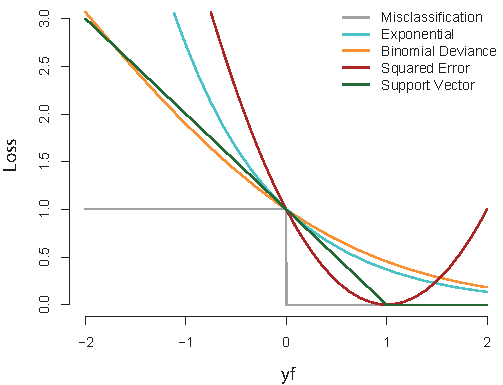
\includegraphics[scale=.5]{images/lossfuncs}}
Which of these might work best may be specific to the situation, but the gist is that they penalize negative values (misclassifications) more heavily and increasingly so the worse the misclassification (except for misclassification error, which penalizes all misclassifications equally), with their primary difference in how heavy that penalty is.  At right is a depiction of the loss as a functions above, taken from \citet{hastie_elements_2009}.






% !Rnw root = ../mlcrash.Rnw





%%%%%%%%%%%%%%%%%%%%%
\part{Regularization}
%%%%%%%%%%%%%%%%%%%%%
\newthought{It is important to note} that a model fit to a single data set might do very well with the data at hand, but then suffer when predicting independent data \sidenote{In terminology we will discuss further later, such models might have low bias but notable variance.}.  Also, oftentimes we are interested in a 'best' subset of predictors among a great many, and in this scenario the estimated coefficients are overly optimistic.  This general issue can be improved by shrinking estimates toward zero, such that some of the performance in the initial fit is sacrificed for improvement with regard to prediction.

Penalized estimation will provide estimates with some shrinkage, and we can use it with little additional effort with our common procedures.  Concretely, let's apply this to the standard linear model, where we are finding estimates of $\beta$ that minimize the squared error loss.

\vspace{.25cm}
$\hat\beta = \underset{\beta}{\mathrm{arg\, min}} \sum{(y-X\beta)^2}$ 
\vspace{.25cm}

In words, we're finding the coefficients that minimize the sum of the squared residuals.  With the approach to regression here we just add a penalty component to the procedure as follows.

\vspace{.25cm}
$\hat\beta = \underset{\beta}{\mathrm{arg\, min}} \sum{(y-X\beta)^2} + \lambda\overset{p}{\underset{j=1}{\sum}}{\left|\beta_j\right|}$ 
\vspace{.25cm}

%
In the above equation, $\lambda$ is our penalty term\sidenote{This can be set explicitly or also estimated via a validation approach.  As we do not know it beforehand, we can estimate it on a validation data set (not the test set) and then use the estimated value when estimating coefficients via cross-validation with the test set.  We will talk more about validation later.} for which larger values will result in more shrinkage.  It's applied to the $L_1$ or Manhattan norm of the coefficients, $\beta_1,\beta_2...\beta_p$, i.e. \emph{not including the intercept} $\beta_0$, and is the sum of their absolute values (commonly referred to as the \emph{lasso}\sidenote{See Tibshirani (1996) Regression shrinkage and selection via the lasso.}). For generalized linear and additive models, we can conceptually express a penalized likelihood as follows:

\vspace{.25cm}
$l_p(\beta) = l(\beta) - \lambda\overset{p}{\underset{j=1}{\sum}}{\left|\beta_j\right|}$ 
\vspace{.25cm}

As we are maximizing the likelihood the penalty is a subtraction, but nothing inherently different is shown.  This basic idea of adding a penalty term will be applied to all machine learning approaches, but as shown, we can apply such a tool to classical methods to boost prediction performance.

It should be noted that we can go about the regularization in different ways.  For example, using the squared $L_2$ norm results in what is called \emph{ridge} regression (a.k.a. Tikhonov regularization)\sidenote{Interestingly, the lasso and ridge regression results can be seen as a Bayesian approach using a zero mean Laplace and Normal prior distribution respectively for the $\beta_j$.}, and using a weighted combination of the lasso and ridge penalties gives us \emph{elastic net} regularization. 

%%%
\section{R Example}
In the following example, we take a look at the lasso approach for a standard linear model.  We add the regularization component, with a fixed penalty $\lambda$ for demonstration purposes\sidenote{As noted previously, in practice $\lambda$ would be estimated via some validation procedure.}.  However you should insert your own values for $\lambda$ in the \texttt{\textcolor{red}{optim}} line to see how the results are affected. 

\vspace{.25cm}
\begin{knitrout}\footnotesize
\definecolor{shadecolor}{rgb}{0.969, 0.969, 0.969}\color{fgcolor}\begin{kframe}
\begin{alltt}
\hlstd{sqerrloss_reg} \hlkwb{=} \hlkwa{function}\hlstd{(}\hlkwc{beta}\hlstd{,} \hlkwc{X}\hlstd{,} \hlkwc{y}\hlstd{,} \hlkwc{lambda}\hlstd{=}\hlnum{.1}\hlstd{)\{}
  \hlstd{mu} \hlkwb{=} \hlstd{X}\hlopt\hlstd{beta}
  \hlkwd{sum}\hlstd{((y}\hlopt{-}\hlstd{mu)}\hlopt{^}\hlnum{2}\hlstd{)} \hlopt{+} \hlstd{lambda}\hlopt{*}\hlkwd{sum}\hlstd{(}\hlkwd{abs}\hlstd{(beta[}\hlopt{-}\hlnum{1}\hlstd{]))}
\hlstd{\}}

\hlstd{out3} \hlkwb{=} \hlkwd{optim}\hlstd{(}\hlkwc{par}\hlstd{=}\hlkwd{c}\hlstd{(}\hlnum{0}\hlstd{,}\hlnum{0}\hlstd{,}\hlnum{0}\hlstd{),} \hlkwc{fn}\hlstd{=sqerrloss_reg,} \hlkwc{X}\hlstd{=X,} \hlkwc{y}\hlstd{=y)}
\hlkwd{rbind}\hlstd{(}\hlkwd{c}\hlstd{(out1}\hlopt{$}\hlstd{par, out1}\hlopt{$}\hlstd{value),}
      \hlkwd{c}\hlstd{(}\hlkwd{coef}\hlstd{(out2),}\hlkwd{sum}\hlstd{(}\hlkwd{resid}\hlstd{(out2)}\hlopt{^}\hlnum{2}\hlstd{)),}
      \hlkwd{c}\hlstd{(out3}\hlopt{$}\hlstd{par, out3}\hlopt{$}\hlstd{value) )}
\end{alltt}
\begin{verbatim}
##      (Intercept) X[, 2] X[, 3]      
## [1,]      0.2702 0.7336  1.048 351.1
## [2,]      0.2701 0.7337  1.048 351.1
## [3,]      0.2704 0.7328  1.047 351.3
\end{verbatim}
\end{kframe}
\end{knitrout}


From the above, we can see in this case that the predictor coefficients have indeed shrunk toward zero slightly while the residual sum of squares has increased just a tad.

In general, we can add the same sort of penalty to any number of models, such as logistic regression, neural net models, recommender systems etc.  The primary goal again is to hopefully increase our ability to generalize the selected model to new data.  Note that the estimates produced are in fact biased, but we have decreased the variance with new predictions as a counterbalance, and this brings us to the topic of the next section.



% !Rnw root = ../mlcrash.Rnw




%%%%%%%%%%%%%%%%%%%%%%%%%%%%%
\part{Bias-Variance Tradeoff}
%%%%%%%%%%%%%%%%%%%%%%%%%%%%%
\newthought{In most of science} we are concerned with reducing uncertainty in our knowledge of some phenomenon.  The more we know about the factors involved or related to some outcome of interest, the better we can predict that outcome upon the influx of new information.  The initial step is to take the data at hand, and determine how well a model or set of models fit the data in various fashions.  In many applications however, this part is also more or less the end of the game as well\sidenote{I should note that I do not make any particular claim about the quality of such analysis.  In many situations the cost of data collection is very high, and for all the current enamorment with 'big' data, a lot of folks will never have access to big data for their situation (e.g. certain clinical populations).  In these situations getting new data for which one might make predictions is extremely difficult.}.

Unfortunately, such an approach in which we only fit models to one data set does not give a very good sense of \emph{generalization} performance, i.e. the performance we would see with new data.  While typically not reported, most researchers, if they are spending appropriate time with the data, are actually testing a great many models, for which the 'best' is then provided in detail in the end report.  Without some generalization performance check however, such performance is overstated when it comes to new data.

In the following consider a standard linear model scenario, e.g. with squared-error loss function and perhaps some regularization, and a data set in which we split the data in some random fashion into a \emph{training} set, for initial model fit, and a \emph{test} set, which is a separate and independent data set, to measure generalization performance\sidenote{In typical situations there are parameters specific to some analytical technique for which one would have no knowledge and which must be estimated along with the usual parameters of the standard models. The $\lambda$ penalty parameter in regularized regression is one example of such a \emph{tuning} parameter. In the best case scenario, we would also have a \emph{validation} set, where we could determine appropriate values for such parameters based on performance with the validation data set, and then assess generalization performance on the test set when the final model has been chosen.  However, methods are available to us in which we can approximate the validation step in other ways.}.  We note \emph{training error} as the (average) loss over the training set, and \emph{test error} as the (average) prediction error obtained when a model resulting from the training data is fit to the test data.  So in addition to the previously noted goal of finding the 'best' model (\emph{model selection}), we are interested further in estimating the prediction error with new data (\emph{model performance}).

%%%
\section{Bias \& Variance}
Conceptually\sidenote{Much of the following is essentially a paraphrase of parts of \citet[Chap. 2 \& 7]{hastie_elements_2009}.}, with the standard model $Y = f(X) + \epsilon$ with we can think of the expected prediction error at a specific input $X = x_0$ as: \\

\vspace{.25cm}
\noindent $\text{Error}_{x_0} = \text{Irreducible Error} + \text{Bias}^2 + \text{Variance}$
\vspace{.25cm}

In other words, we have three components to our general notion of prediction error: \\

\begin{description}
  \item[$\sigma^2_\epsilon$] An initial variance of the target around the true mean $f(x_0)$ (unavoidable).
  \item[$Bias^2$] the amount the \emph{average} of our estimate varies from the true mean.
  \item[Variance] the variance of the target value about its mean.
\end{description}

Slightly more formally, we can present this as follows, with $h_0$ our estimated (hypothesized) value:

\vspace{.25cm}
\noindent $\text{Error}_{x_0} = Var(\epsilon) + (\text{E}[h_0] - f(x_0))^2 + Var(h_0) $
\vspace{.25cm}


%%%
\section{The Tradeoff}
Outlining a general procedure, we start by noting the prediction error on a training data set with multiple models of varying complexity (e.g. increasing the number of predictor variables), and then assess the performance of the chosen models in terms of prediction error on the test set.  We then perform the same activity for a total of 100 simulated data sets, for each level of complexity.

\marginnote{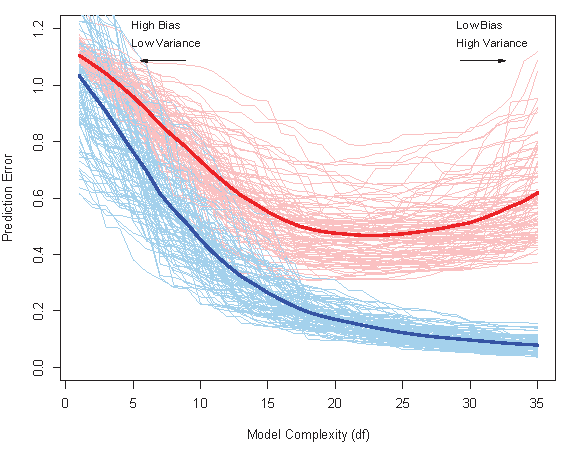
\includegraphics[scale=.5]{images/biasvar2}}The results from this process might look like the image to the right taken from \citet{hastie_elements_2009}.  With regard to the training data, we have $error_{train}$ for one hundred training sets for each level of model complexity.  The bold blue line notes this average error over the 100 sets by model complexity.  The bold red line the average test error ($error_{test}$) across the 100 test data sets.

Ideally we'd like to see low bias and variance, but things are not so easy. One thing we can see clearly is that $error_{train}$ is not a good estimate of $error_{test}$, which is now our focus in terms of performance. If we think of the training error as what we would see in typical research where one does everything with a single data set, we are using the same data set to fit the model and assess error.  As the model is adapted to that data set specifically, it will be overly optimistic in the estimate of the error, that optimism being the difference between the error rate we see based on the training data versus the average of what we would get with many test data sets.  We can think of this as a problem of overfitting to the training data.  Models that do not incorporate any regularization or validation process of any kind are likely overfit to the data presented.

Generally speaking, the more complex the model, the lower the bias, but the higher the variance, as depicted in the graphic.  Specifically however, the situation is more nuanced, where type of problem (classification with 0-1 loss vs. continuous response with squared error loss\sidenote{See Friedman (1996) \emph{On Bias, Variance, 0/1 Loss and the Curse of Dimensionality} for the unusal situations that can arise in dealing with classification error with regard to bias and variance.}) and technique (a standard linear model vs. regularized fit) will exhibit different bias-variance relationships.

%%%
\section{Diagnosing Bias-Variance Issues \& Possible Solutions}
Let's assume a regularized linear model with a standard data split into training and test sets.  We will describe different scenarios with possible solutions.

\marginnote{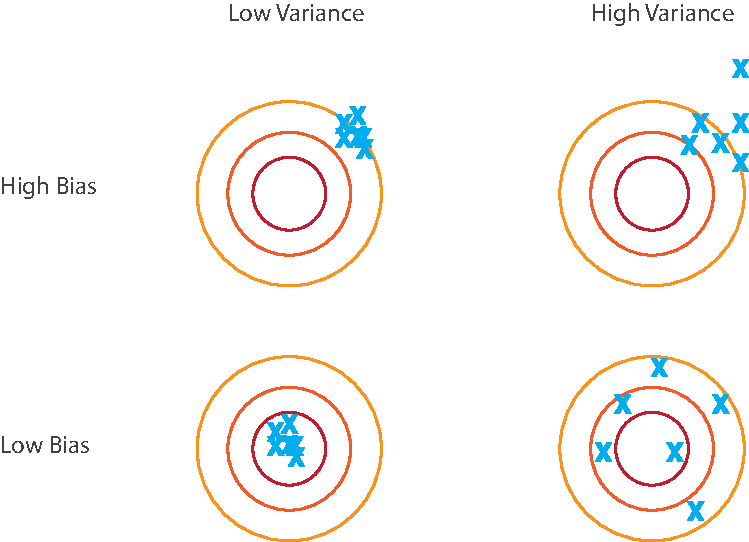
\includegraphics[scale=.35]{images/biasvartarget} \footnotesize{Figure adapted from \citet{domingos_few_2012}.}}
\subsection{Worst Case Scenario}
Starting with the worst case scenario, poor models may exhibit high bias and high variance.  One thing that will not help this situation (perhaps contrary to intuition) is adding more data, i.e. increasing N.  You can't make a silk purse out of a sow's ear (\emph{usually}\sidenote{\url{https://libraries.mit.edu/archives/exhibits/purse/}}), and adding more data just gives you a more accurate picture of how awful your model is. One might need to rework the model, e.g. adding new predictors or creating them via interaction terms, polynomials, or other smooth functions as in additive models, or simply collecting better and/or more relevant data.\marginnote{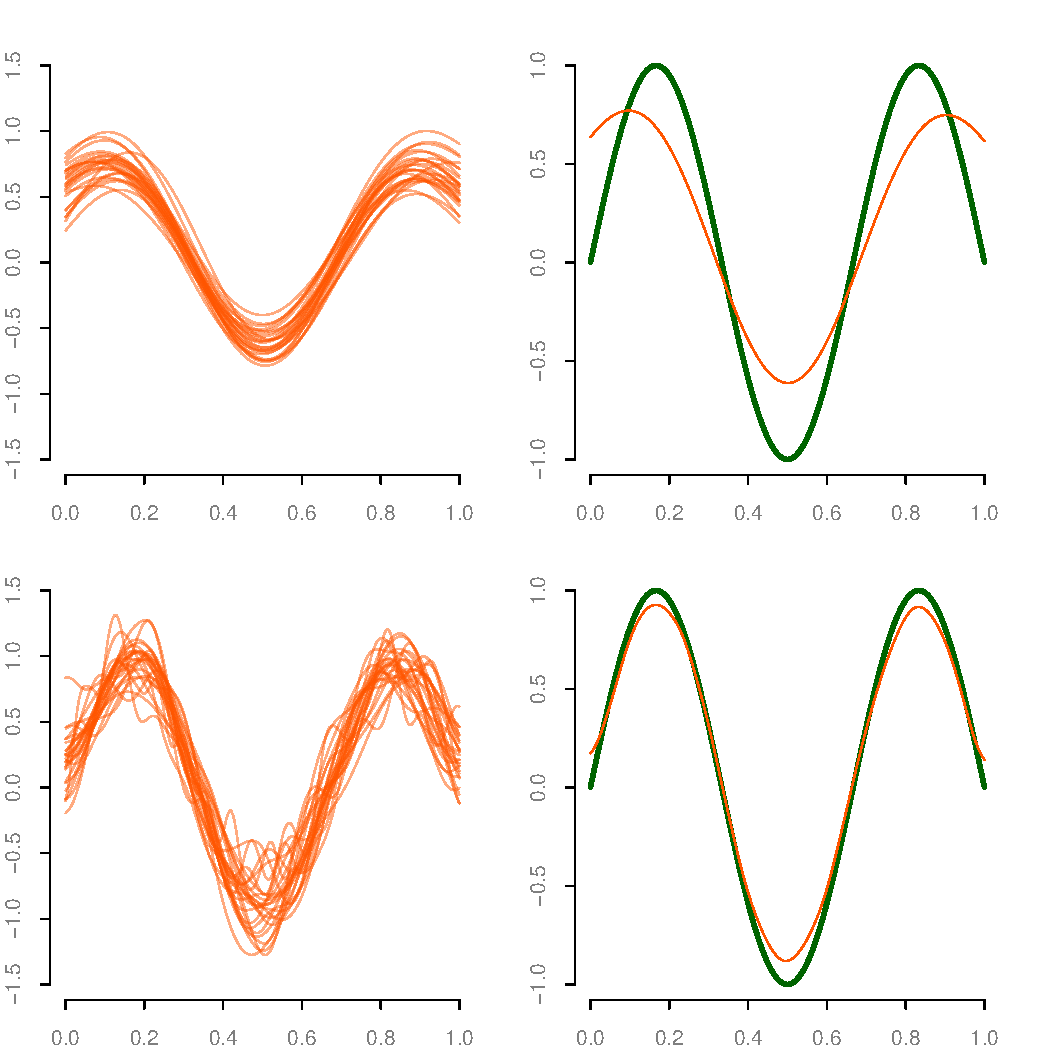
\includegraphics[scale=.35]{images/graph64} \footnotesize{Figure inspired by \citet[figure 6.5]{murphy_machine_2012} showing the bias-variance tradeoff.  Sample (left) and average (right) fits of linear regression using a gaussian radial basis function expansion. The green line represents the true relationship. The top row shows low variance between one fit and the next (left) but notable bias (right) in that the average fit is off.  Compare to the less regularized (high variance, low bias) situation of the bottom row.  See the \emph{\textcolor{blue}{kernlab}} package for the fitting function used.}}


\subsection{High Variance}
When variance is a problem, our training error is low while test error is relatively high (overfitting problem). Implementing more shrinkage or other penalization to model complexity may help with the issue.  In this case more data may help as well.

\subsection{High Bias}
With bias issues our training error is high and test error is not too different from training error (underfitting problem).  Adding new predictors/features, interaction terms, polynomials etc. can help here.  Additionally reducing the penalty parameter $\lambda$ would also work with even less effort, though generally it should be estimated rather than explicitly set.



% !Rnw root = ../mlcrash.Rnw




%%%%%%%%%%%%%%%%%%%%%%%
\part{Cross-Validation}
%%%%%%%%%%%%%%%%%%%%%%%
As noted in the previous section, in machine learning approaches we are particularly concerned with prediction error on new data.  The simplest validation approach would be to split the data available into a training and test set as discussed previously.  We estimate the model on the training data, and apply the model to the test data, get the predictions and measure our test error, selecting whichever model results in the least test error.  \marginnote{\center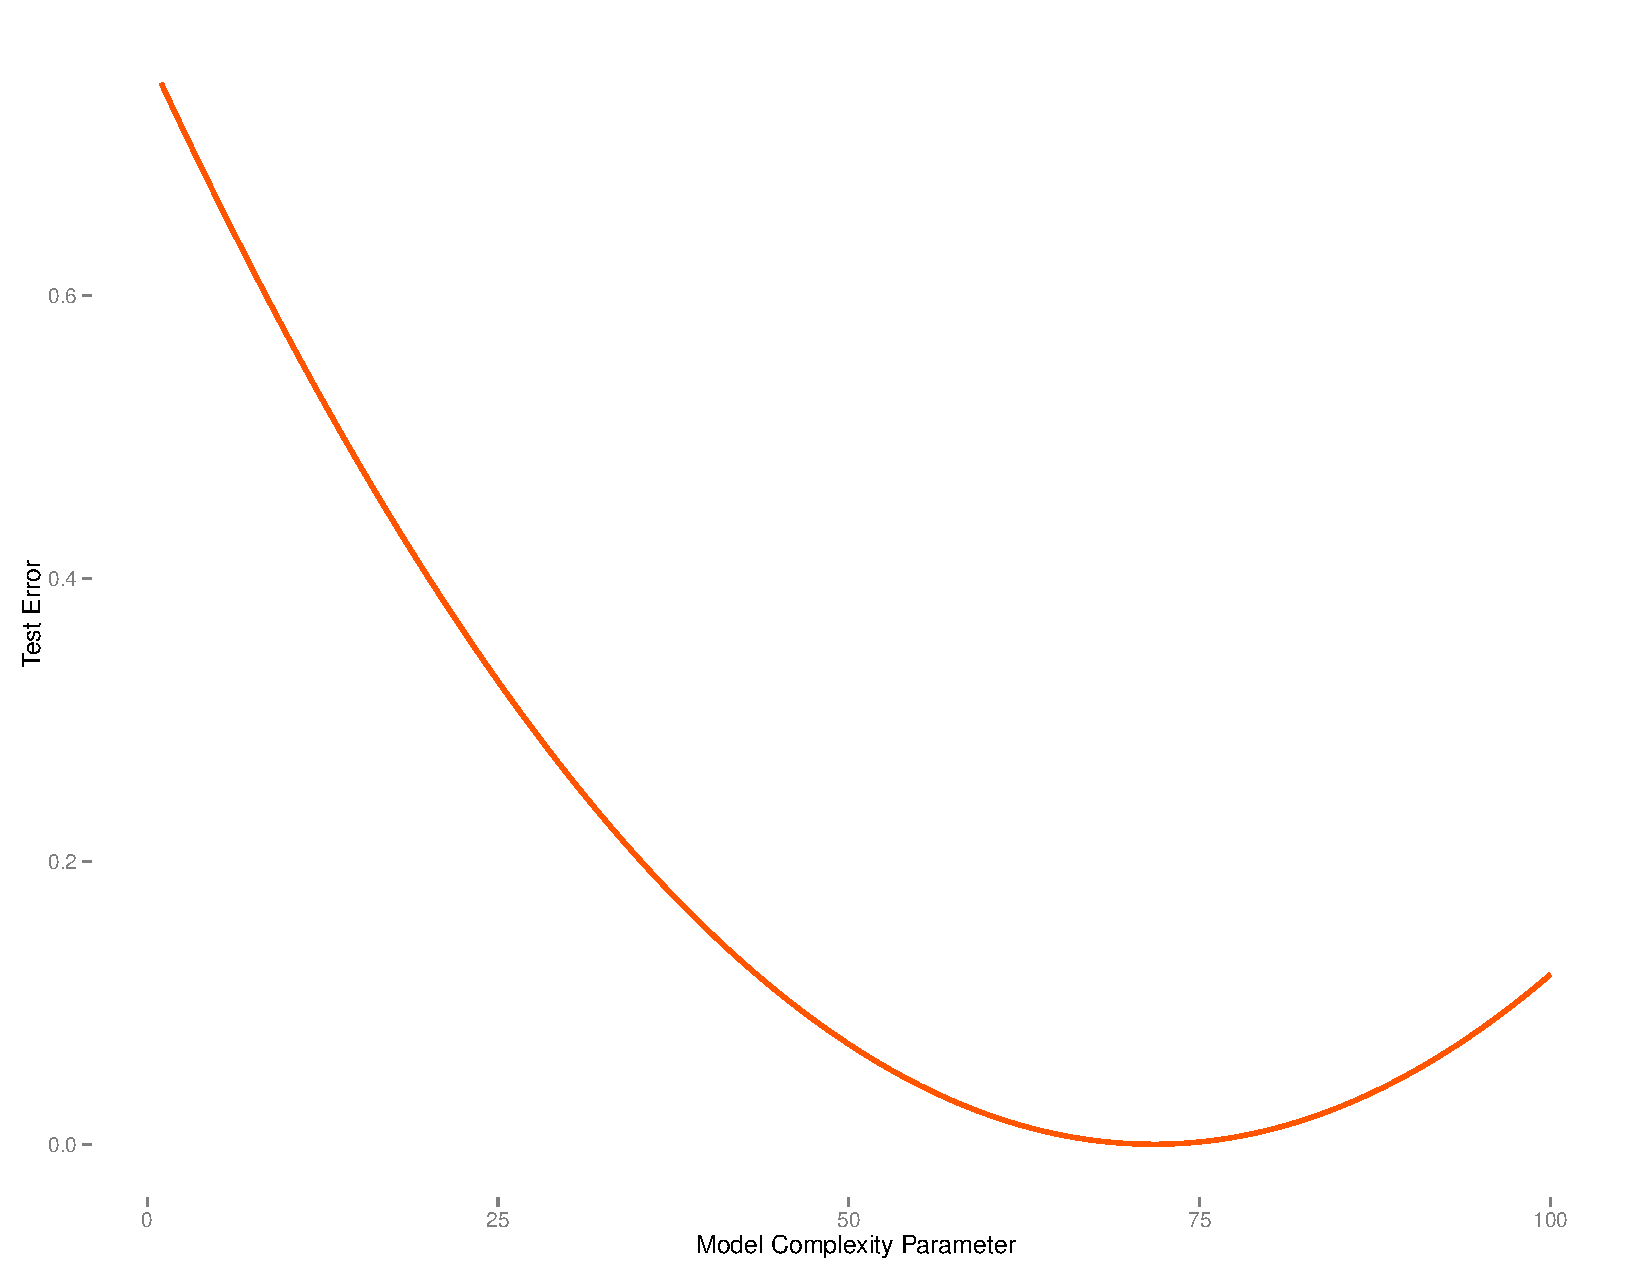
\includegraphics[scale=.2]{images/learningcurve.pdf}}A hypothetical learning curve display the results of such a process is shown to the right. While fairly simple, other approaches are more commonly used and result in better estimates of performance\sidenote{Along with some of the other works cited, see \citet{harrell_regression_2001} for a good discussion of model validation.}.

\section{Adding Another Validation Set}
One technique that might be utilized for larger data sets, is to split the data into training, validation and final test sets.  For example, one might take the original data and create something like a 60-20-20\% split to create the needed data sets.  The purpose of the initial validation set is to select the optimal model and determine the values of tuning parameters.  These are parameters which generally deal with how complex a model one will allow, but for which one would have little inkling as to what they should be set at before hand (e.g. our $\lambda$ shrinkage parameter).  We select models/tuning parameters that minimize the validation set error, and once the model is chosen examine test set error performance.  In this way performance assessment is still independent of the model development process.

\section{K-fold Cross-Validation}
\marginnote{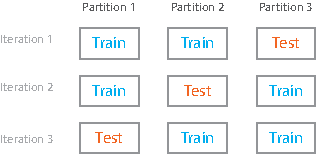
\includegraphics[scale=1]{images/kfold.pdf} \vspace{.5cm} \\ An illustration of 3-fold classification.}In many cases we don't have enough data for such a split, and the split percentages are arbitrary anyway and results would be specific to the specific split chosen.  Instead we can take a typical data set and randomly split it into $\kappa=10$ equal-sized (or close to it) parts.  Take the first nine partitions and use them as the training set.  With chosen model, make predictions on the test set.  Now do the same but this time use the 9th partition as the holdout set. Repeat the process until each of the initial 10 partitions of data have been used as the test set.  Average the error across all procedures for our estimate of prediction error.  With enough data, this (and the following methods) could be used as the validation procedure before eventual performance assessment on an independent test set with the final chosen model.

\subsection{Leave-one-out Cross-Validation}
Leave-one-out (LOO) cross-validation is pretty much the same thing but where $\kappa=N$.  In other words, we train a model for all observations except the $\kappa^{th}$ one, assessing fit on the observation that was left out. We then cycle through until all observations have been left out once to obtain an average accuracy.  

Of the two, K-fold may have relatively higher bias but less variance, while LOO would have the converse problem, as well as possible computational issues\sidenote{For squared-error loss situations, there is a Generalized cross-validation (GCV) that can be estimated more directly without actually going to the entire LOO procedure, and functions similarly to AIC.}.  K-fold's additional bias would be diminished would with increasing sample sizes, and generally 5 or 10-fold cross-validation is recommended.

\section{Bootstrap}
With a bootstrap approach, we draw $B$ random samples with replacement from our original data set, creating $B$ bootstrapped data sets of the same size as the original data.  We use the $B$ data sets as training sets and, using the original data as the test set, average the prediction error across the models.

\section{Other Stuff}
Along with the above there are variations such as repeated cross validation, the '.632' bootstrap and so forth.  One would want to do a bit of investigating, but $\kappa$-fold and bootstrap approaches generally perform well.  If variable selection is part of the goal, one should be selecting subsets of predictors as part of the cross-validation process, not at some initial data step.




% !Rnw root = ../mlcrash.Rnw




%%%%%%%%%%%%%%%%%%%%%%%%%%%%%%%%%%%%
\part{Model Assessment \& Selection}
%%%%%%%%%%%%%%%%%%%%%%%%%%%%%%%%%%%%

\newthought{In typical model comparison} within the standard linear model framework, there are a number of ways in which we might assess performance across competing models.  For standard OLS regression we might examine adjusted-$R^2$, or with the generalized linear models we might pick a model with the lowest AIC\sidenote{In situations where it is appropriate to calculate in the first place, AIC can often compare to the bootstrap and k-fold cross-validation approaches.}.  As we have already discussed, in the machine learning context we are interested in models that reduce e.g. squared error loss (regression) or misclassification error (classification).  However in dealing with many models some differences in performance may be arbitrary.

%%%
\subsection{Beyond Classification Accuracy: Other Measures of Performance}
In typical classification situations we are interested in overall accuracy.  However there are situations, not uncommon, in which simple accuracy isn't a good measure of performance.  As an example, consider the prediction of the occurrence of a rare disease. Guessing a non-event every time might result in 99.9\% accuracy, but that isn't how we would prefer to go about assessing some classifier's performance.
To demonstrate other sources of classification information, we will use the following 2x2 table that shows values of some binary outcome (0 = non-event, 1 = event occurs) to the predictions made by some model for that response (arbitrary model).  Both a table of actual values, often called a \emph{confusion matrix}\sidenote{This term has always struck me as highly sub-optimal.}, and an abstract version are provided.


\begin{table}[ht]
\begin{minipage}[b]{0.45\linewidth}
    \begin{tabular}{llrr}
     & & & Actual \\
     \hline
     & & 1 & 0\\ 
     \hline
     Predicted & 1 &  41 &  21 \\ 
     & 0 &  16 &  13\\ 
     \hline
    \end{tabular}
\end{minipage}
\hspace{0.5cm}
\begin{minipage}[b]{0.45\linewidth}
    \begin{tabular}{lrrr}
     & & & Actual \\
     \hline
     & & 1 & 0\\ 
     \hline
     Predicted & 1 &  A &  B \\ 
     & 0 &  C &  D\\ 
     \hline
    \end{tabular}
\end{minipage}
\end{table}

\small
\begin{description}
  \item[True Positive, False Positive, True Negative, False Negative] Above, these are A, B, D, and C respectively.
  \item[Accuracy] Number of correct classifications out of all predictions ((A+D)/Total). In the above example this would be (41+13)/91, about 59\%.
  \item[Error Rate] 1 - Accuracy.
  \item[Sensitivity] is the proportion of correctly predicted positives to all true positive events: A/(A+C).  In the above example this would be 41/57, about 72\%. High sensitivity would suggest a low type II error rate (see below), or high statistical \emph{power}. Also known as true positive rate.
  \item[Specificity] is the proportion of correctly predicted negatives to all true negative events: D/(B+D).  In the above example this would be 13/34, about 38\%. High specificity would suggest a low type I error rate (see below). Also known as true negative rate.
  \item[Postive Predictive Value (PPV)] proportion of true positives of those that are predicted positives: A/A+B. In the above example this would be 41/62, about 66\%.
  \item[Negative Predictive Value (NPV)] proportion of true negatives of those that are predicted negative: D/C+D. In the above example this would be 13/29, about 45\%.
  \item[Precision]  See PPV.
  \item[Recall] See sensitivity. 
  \item[Lift] Ratio of positive predictions given actual positives to the proportion of positive predictions out of the total: (A/(A+C))/((A+B)/Total). In the above example this would be (41/(41+16))/((41+21)/(91)), or 1.05.
  \item[F Score (F1 score)] Harmonic mean of precision and recall: 2*(Precision*Recall)/(Precision+Recall). In the above example this would be 2*(.66*.72)/(.66+.72), about .69.  
  \item[Type I Error Rate (false positive rate)] proportion of true negatives that are incorrectly predicted positive: B/B+D. In the above example this would be 21/34, about 62\%.  Also known as alpha.
  \item[Type II Error Rate (false negative rate)] proportion of true positives that are incorrectly predicted negative: C/C+A. In the above example this would be 16/57, about 28\%. Also known as beta.
  \item[False Discovery Rate] proportion of false positives among all positive predictions: B/A+B. In the above example this would be 21/62, about 34\%.  Often used in multiple comparison testing in the context of ANOVA.
  \item[Phi coefficient] A measure of association: (A*D - B*C)/(sqrt((A+C)*(D+B)*(A+B)*(D+C))).  In the above example this would be .11.
\end{description}
\normalsize

Note the following summary of several measures where $N_+$ and $N_-$ are the total true positive values and total true negative values respectively, and $T_+$, $F_+$, $T_-$ and $F_-$ are true positive, false positive, etc.\sidenote{Table based on table 5.3 in \citet{murphy_machine_2012}}:
\vspace{.25cm}

{\footnotesize
\noindent\begin{tabular}{llll}
&  & Actual  & \\
& & 1 & 0 \\
\hline
Predicted & 1 & $T_+/N_+$ = TPR = sensitivity = recall & $F_+/N_-$ = FPR = Type I \\
& 0 & $F_-/N_+$ = FNR = Type II & $T_-/N_-$ = TNR = specificity \\
\hline
\end{tabular} 
}


\vspace{.25cm}
There are many other measures such as area under a Receiver Operating Curve (ROC), odds ratio, and even more names for some of the above.  The gist is that given any particular situation you might be interested in one or several of them, and it would generally be a good idea to look at a few.



% !Rnw root = ../mlcrash.Rnw




%%%%%%%%%%%%%%%%%%%%%%%%%%
\part{Process Overview}
%%%%%%%%%%%%%%%%%%%%%%%%%%
\newthought{Despite the facade of a polished product} one finds in published research, most of the approach with the statistical analysis of data is full of data preparation, starts and stops, debugging, re-analysis, tweaking and fine-tuning etc. Statistical learning is no different in this sense.  Before we begin with explicit examples, it might be best to give a general overview of the path we'll take.

\section{Data Preparation}
As with any typical statistical project, probably most of the time will be spent preparing the data for analysis.  Data is never ready to analyze right away, and careful checks must be made in order to ensure the integrity of the information.  This would include correcting errors of entry, noting extreme values, possibly imputing missing data and so forth.  In addition to these typical activities, we will discuss a couple more things to think about during this initial data examination when engaged in machine learning.

\subsection{Define Data and Data Partitions}
As we have noted previously, ideally we will have enough data to create a \emph{hold-out}, \emph{test}, or \emph{validation} data set. This would be some random partition of the data such that we could safely conclude that the data in the test set comes from the same population as the training set. The training set is used to fit the initial models at various tuning parameter settings, with a 'best' model being that which satisfies some criterion on the validation set (or via a general validation process).  With final model and parameters chosen, generalization error will be assessed with the the performance of the final model on the test data.

\subsection{Feature Scaling}
Even with standard regression modeling, centering continuous variables (subtracting the mean) is a good idea so that intercepts and zero points in general are meaningful. Standardizing variables so that they have similar variances or ranges will help some procedures find their minimums faster.  Another common transformation is \emph{min-max} normalization\sidenote{\footnotesize{$score_{new} = \frac{score_{old}-min_{old}} {max_{old}-min_{old}} (max_{new}-min_{new})+min_{new}$ }}, which will transfer a scale to a new one of some chosen minimum and maximum.  Note that whatever approach is done, it must be done \emph{after} any explicit separation of data.  So if you have separate training and test sets, they should be scaled separately.

\subsection{Feature Engineering}
If we're lucky we'll have ideas on potential combinations or other transformations of the predictors we have available.  For example, in typical social science research there are two-way interactions one is often predisposed to try, or perhaps one can sum multiple items to a single scale score that may be more relevant.  Another common technique is to use a dimension reduction scheme such as principal components, but this can (and probably should) actually be an implemented algorithm in the ML process\sidenote{For example, via principal components or partial least squares regression.}.

One can implement a variety of such approaches in ML as well to create additional potentially relevant features, even automatically, but as a reminder, a key concern is overfitting, and doing broad construction of this sort with no contextual guidance would potentially be prone to such a pitfall.  In other cases it may simply be not worth the time expense.

\subsection{Discretization}
While there may be some contextual exceptions to the rule, it is generally a pretty bad idea in standard statistical modeling to discretize/categorize continuous variables\sidenote{See \citet{harrell_regression_2001} for a good summary of reasons why not to.}.  However some ML procedures will work better (or just faster) if dealing with discrete valued predictors rather than continuous. Others even require them; for example, logic regression needs binary input.  While one could pick arbitrary intervals and cutpoints in an unsupervised fashion such as picking equal range bins or equal frequency bins, there are supervised algorithmic approaches that will use the information in the data to produce some 'optimal' discretization.

It's generally not a good idea to force things in data analysis, and given that a lot of data situations will be highly mixed, it seems easier to simply apply some scaling to preserve the inherent relationships in the data.  Again though, if one has only a relative few continuous variables or a context in which it makes sense to, it's probably better to leave continuous variables as such.

\section{Model Selection}
With data prepared and ready to analyze, one can use a validation process to come up with a viable model.  Use an optimization procedure or a simple grid search over a set of specific values to examine models at different tuning parameters. Perhaps make a finer search once an initial range of good performing values is found, though one should not split hairs over arbitrarily close performance.  Select a 'best' model given some criterion such as overall accuracy, or if concerned about over fitting, select the simplest model within one standard error of the accuracy of the best, or perhaps the simplest within X\% of the best model.  For highly skewed classes, one might need to use a different measure of performance besides accuracy.  If one has a great many predictor variables, one may use the model selection process to select features that are 'most important'.

\section{Model Assessment}
With tuning parameters/features chosen, we then examine performance on the independent test set (or via some validation procedure). For classification problems, consider other statistics besides accuracy as measures of performance, especially if classes are unbalanced. Consider other analytical techniques that are applicable and compare performance among the different approaches.  One can even combine disparate models' predictions to possibly create an even better classifier\sidenote{The topic of ensembles is briefly noted later.}.



% !Rnw root = ../mlcrash.Rnw





%%%%%%%%%%%%%%%%%%%%%%%%%%%%
\part{Opening the Black Box}
%%%%%%%%%%%%%%%%%%%%%%%%%%%%

\newthought{It's now time to see some of this in action}.  In the following we will try a variety of techniques so as to get a better feel for the sorts of things we might try out.

\section{The Dataset}
We will use the wine data set from the UCI Machine Learning data repository.  The goal is to predict wine quality, of which there are 7 values (integers 3-9).  We will turn this into a binary classification task to predict whether a wine is 'good' or not, which is arbitrarily chosen as 6 or higher.  After getting the hang of things one might redo the analysis as a multiclass problem or even toy with regression approaches, just note there are very few 3s or 9s so you really only have 5 values to work with.  The original data along with detailed description can be found \href{http://archive.ics.uci.edu/ml/datasets/Wine+Quality}{here}, but aside from quality it contains predictors such as residual sugar, alcohol content, acidity and other characteristics of the wine\sidenote{I think it would be interesting to have included characteristics of the people giving the rating.}.

The original data is separated into white and red data sets. I have combined them and created additional variables: \emph{color} and its numeric version \emph{white} indicating white or red, and \emph{good}, indicating scores greater than or equal to 6 (denoted as 'Good').  The following will show some basic numeric information about the data.

\begin{knitrout}\footnotesize
\definecolor{shadecolor}{rgb}{0.969, 0.969, 0.969}\color{fgcolor}\begin{kframe}
\begin{alltt}
\hlstd{wine} \hlkwb{=} \hlkwd{read.csv}\hlstd{(}\hlstr{"http://www.nd.edu/~mclark19/learn/data/goodwine.csv"}\hlstd{)}
\hlkwd{summary}\hlstd{(wine)}
\end{alltt}
\begin{verbatim}
##  fixed.acidity   volatile.acidity  citric.acid    residual.sugar 
##  Min.   : 3.80   Min.   :0.08     Min.   :0.000   Min.   : 0.60  
##  1st Qu.: 6.40   1st Qu.:0.23     1st Qu.:0.250   1st Qu.: 1.80  
##  Median : 7.00   Median :0.29     Median :0.310   Median : 3.00  
##  Mean   : 7.21   Mean   :0.34     Mean   :0.319   Mean   : 5.44  
##  3rd Qu.: 7.70   3rd Qu.:0.40     3rd Qu.:0.390   3rd Qu.: 8.10  
##  Max.   :15.90   Max.   :1.58     Max.   :1.660   Max.   :65.80  
##    chlorides     free.sulfur.dioxide total.sulfur.dioxide    density     
##  Min.   :0.009   Min.   :  1.0       Min.   :  6          Min.   :0.987  
##  1st Qu.:0.038   1st Qu.: 17.0       1st Qu.: 77          1st Qu.:0.992  
##  Median :0.047   Median : 29.0       Median :118          Median :0.995  
##  Mean   :0.056   Mean   : 30.5       Mean   :116          Mean   :0.995  
##  3rd Qu.:0.065   3rd Qu.: 41.0       3rd Qu.:156          3rd Qu.:0.997  
##  Max.   :0.611   Max.   :289.0       Max.   :440          Max.   :1.039  
##        pH         sulphates        alcohol        quality       color     
##  Min.   :2.72   Min.   :0.220   Min.   : 8.0   Min.   :3.00   red  :1599  
##  1st Qu.:3.11   1st Qu.:0.430   1st Qu.: 9.5   1st Qu.:5.00   white:4898  
##  Median :3.21   Median :0.510   Median :10.3   Median :6.00               
##  Mean   :3.22   Mean   :0.531   Mean   :10.5   Mean   :5.82               
##  3rd Qu.:3.32   3rd Qu.:0.600   3rd Qu.:11.3   3rd Qu.:6.00               
##  Max.   :4.01   Max.   :2.000   Max.   :14.9   Max.   :9.00               
##      white         good     
##  Min.   :0.000   Bad :2384  
##  1st Qu.:1.000   Good:4113  
##  Median :1.000              
##  Mean   :0.754              
##  3rd Qu.:1.000              
##  Max.   :1.000
\end{verbatim}
\end{kframe}
\end{knitrout}



\section{R Implementation}
I will use the \emph{\textcolor{blue}{caret}} package in R.  Caret makes implementation of validation, data partitioning, performance assessment, and prediction and other procedures about as easy as it can be in this environment.  However, caret is mostly using other R packages\sidenote{In the following, the associated packages and functions used are: 
\begin{description}
  \item[\textcolor{blue}{caret}] \textcolor{red}{knn}
  \item[\textcolor{blue}{nnet}] \textcolor{red}{nnet} 
  \item[\textcolor{blue}{randomForest}] \textcolor{red}{randomForest}
  \item[\textcolor{blue}{kernlab}] \textcolor{red}{ksvm} 
\end{description}
} that have more information about the specific functions underlying the process, and those should be investigated for additional information.  Check out the \href{http://caret.r-forge.r-project.org/}{caret home page} for more detail. The methods selected here were chosen for breadth of approach, to give a good sense of the variety of techniques available.

In addition to caret, it's a good idea to use your computer's resources as much as possible, or some of these procedures may take a notably long time, and more so with the more data you have.  Caret will do this behind the scenes, but you first need to set things up. Say, for example, you have a quad core processor, meaning your processor has four cores essentially acting as independent CPUs. You can set up R for parallel processing with the following code, which will allow caret to allot tasks to three cores simultaneously\sidenote{You typically want to leave at least one core free so you can do other things.}.

%%% put cache to FALSE here if rerunning models to utilize additional cpu %%%
\begin{knitrout}\footnotesize
\definecolor{shadecolor}{rgb}{0.969, 0.969, 0.969}\color{fgcolor}\begin{kframe}
\begin{alltt}
\hlkwd{library}\hlstd{(doSNOW)}
\hlkwd{registerDoSNOW}\hlstd{(}\hlkwd{makeCluster}\hlstd{(}\hlnum{3}\hlstd{,} \hlkwc{type} \hlstd{=} \hlstr{"SOCK"}\hlstd{))}
\end{alltt}
\end{kframe}
\end{knitrout}


\section{Feature Selection \& The Data Partition}
This data set is large enough to leave a holdout sample, allowing us to initially search for the best of a given modeling approach over a grid of tuning parameters specific to the technique.  To iterate previous discussion, we don't want test performance contaminated with the tuning process.  With the best model at $t$ tuning parameter(s), we will assess performance with prediction on the holdout set.

\marginnote{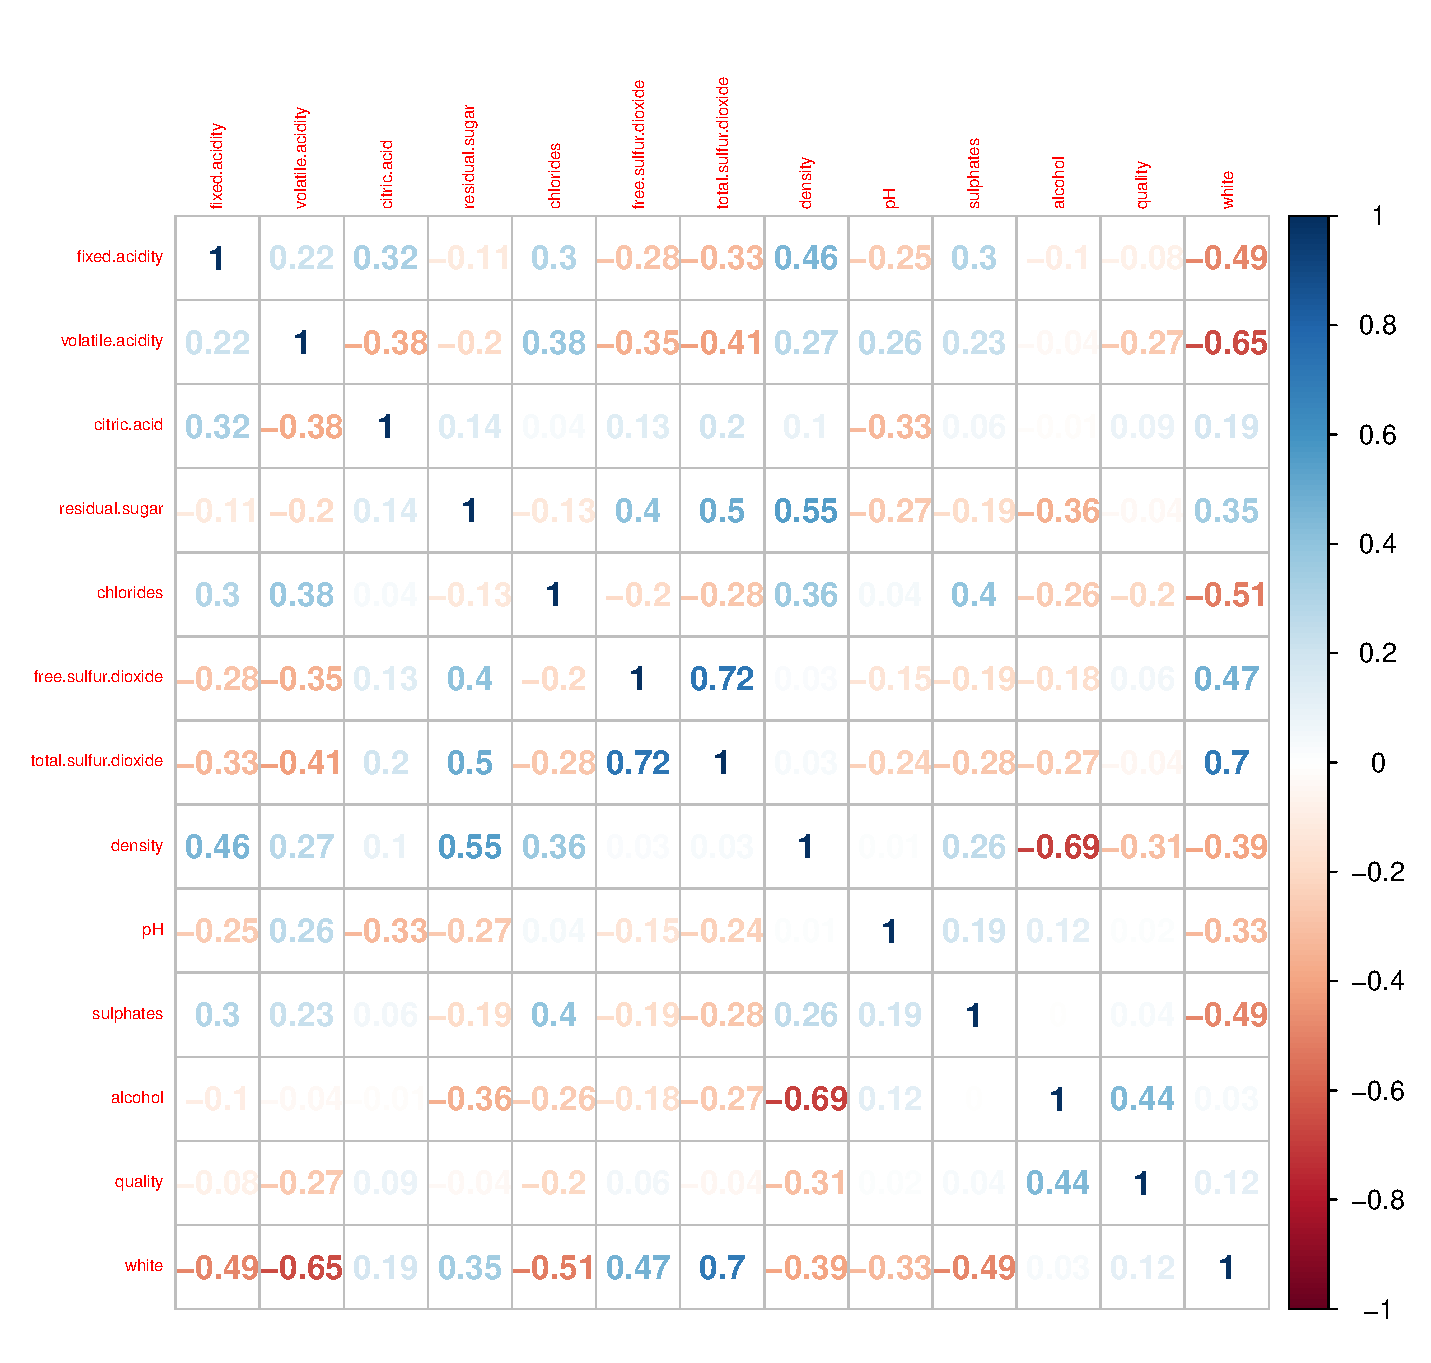
\includegraphics[scale=.25]{images/corrplot}}
I also made some decisions to deal with the notable collinearity in the data, which can severely hamper some methods.  We can look at the simple correlation matrix to start

\begin{knitrout}\footnotesize
\definecolor{shadecolor}{rgb}{0.969, 0.969, 0.969}\color{fgcolor}\begin{kframe}
\begin{alltt}
\hlkwd{library}\hlstd{(corrplot)}
\hlkwd{corrplot}\hlstd{(}\hlkwd{cor}\hlstd{(wine[,} \hlopt{-}\hlkwd{c}\hlstd{(}\hlnum{13}\hlstd{,} \hlnum{15}\hlstd{)]),} \hlkwc{method} \hlstd{=} \hlstr{"number"}\hlstd{,} \hlkwc{tl.cex} \hlstd{=} \hlnum{0.5}\hlstd{)}
\end{alltt}
\end{kframe}
\end{knitrout}


I ran regressions to examine the r-squared for each predictor in a model as if it were the dependent variable predicted by the other input variables.  The highest was for density at over 96\%, and further investigation suggested color and either sulfur dioxide are largely captured by the other variables already also.  These will not be considered in the following models.

Caret has its own partitioning function we can use here to separate the data into training and test data.  There are 6497 total observations of which I will put 80\% into the training set.  The function \textcolor{red}{createDataPartition} will produce indices to use as the training set.  In addition to this, we will normalize the continuous variables to the [0,1] range.  For the training data set, this will be done as part of the training process, so that any subsets under consideration are scaled separately, but for the test set we will go ahead and do it now.

\begin{knitrout}\footnotesize
\definecolor{shadecolor}{rgb}{0.969, 0.969, 0.969}\color{fgcolor}\begin{kframe}
\begin{alltt}
\hlkwd{library}\hlstd{(caret)}
\hlkwd{set.seed}\hlstd{(}\hlnum{1234}\hlstd{)}  \hlcom{#so that the indices will be the same when re-run}
\hlstd{trainIndices} \hlkwb{=} \hlkwd{createDataPartition}\hlstd{(wine}\hlopt{$}\hlstd{good,} \hlkwc{p} \hlstd{=} \hlnum{0.8}\hlstd{,} \hlkwc{list} \hlstd{= F)}
\hlstd{wanted} \hlkwb{=} \hlopt{!}\hlkwd{colnames}\hlstd{(wine)} \hlopt \hlkwd{c}\hlstd{(}\hlstr{"free.sulfur.dioxide"}\hlstd{,} \hlstr{"density"}\hlstd{,} \hlstr{"quality"}\hlstd{,}
    \hlstr{"color"}\hlstd{,} \hlstr{"white"}\hlstd{)}
\hlstd{wine_train} \hlkwb{=} \hlstd{wine[trainIndices, wanted]}  \hlcom{#remove quality and color, as well as density and others}

\hlstd{wine_test} \hlkwb{=} \hlstd{wine[}\hlopt{-}\hlstd{trainIndices, wanted]}
\end{alltt}
\end{kframe}
\end{knitrout}


\marginnote{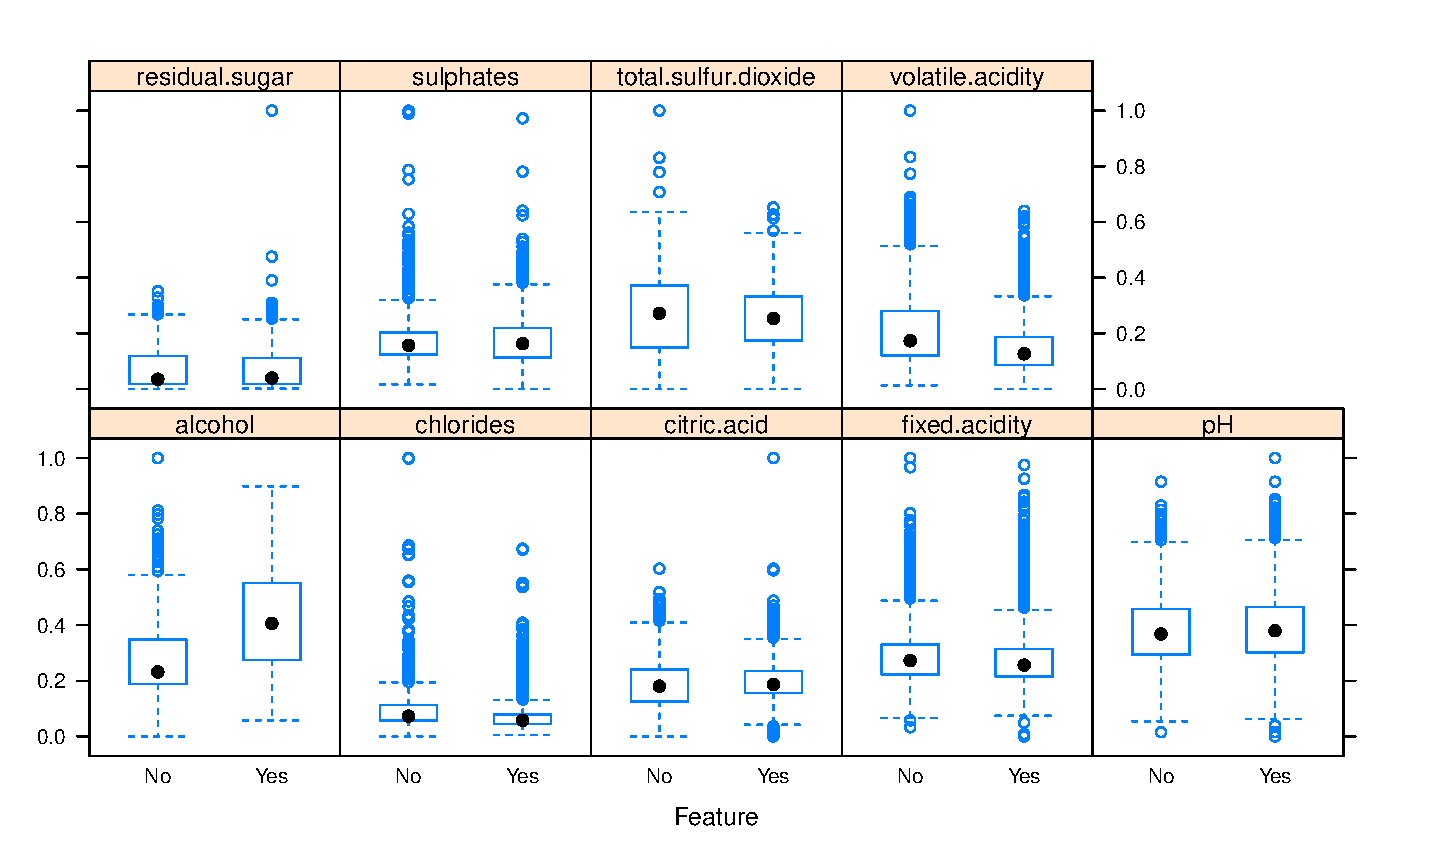
\includegraphics[scale=.25]{images/classbox}}
Let's take an initial peek at how the predictors separate on the target.  In the following I'm 'predicting' the pre-possessed data so as to get the transformed data.  Again, we'll leave the preprocessing to the training part, but here it will put them on the same scale for visual display. 

\begin{knitrout}\footnotesize
\definecolor{shadecolor}{rgb}{0.969, 0.969, 0.969}\color{fgcolor}\begin{kframe}
\begin{alltt}
\hlstd{wine_trainplot} \hlkwb{=} \hlkwd{predict}\hlstd{(}\hlkwd{preProcess}\hlstd{(wine_train[,}\hlopt{-}\hlnum{10}\hlstd{],} \hlkwc{method}\hlstd{=}\hlstr{"range"}\hlstd{),}
                         \hlstd{wine_train[,}\hlopt{-}\hlnum{10}\hlstd{])}
\hlkwd{featurePlot}\hlstd{(wine_trainplot, wine_train}\hlopt{$}\hlstd{good,} \hlstr{"box"}\hlstd{)}
\end{alltt}
\end{kframe}
\end{knitrout}


For the training set, it looks like alcohol content, volatile acidity and chlorides separate most with regard to good classification. While this might give us some food for thought, note that the figure does not give insight into interaction effects, which methods such as trees will get at.

%%%
\section{$k$-nearest Neighbors}
Consider the typical distance matrix\sidenote{See, for example, the function \textcolor{red}{dist} in R.} that is often used for cluster analysis of observations\sidenote{Often referred to as \emph{unsupervised} learning as there is not target/dependent variable.}. If we choose something like \emph{Euclidean distance} as a metric, each point in the matrix gives the value of how far an observation is from some other, given their respective values on a set of variables.

K-nearest neighbors approaches exploit this information for predictive purposes.  Let us take a classification example, and $k = 5$ neighbors.  For a given observation $x_i$, find the 5 closest neighbors in terms of Euclidean distance based on the predictor variables.  The class that is predicted is whatever class the majority of the neighbors are labeled as\sidenote{See the \textcolor{red}{knn.ani} function in the \textcolor{blue}{animation} package for a visual demonstration}.  For continuous outcomes we might take the mean of those neighbors as the prediction.

So how many neighbors would work best? This is an example of a tuning parameter, i.e. $k$, for which we have no knowledge about its value without doing some initial digging.  As such we will select the tuning parameter as part of the validation process.

The caret package provides several techniques for validation such as $k$-fold, bootstrap, leave-one-out and others.  We will use 10-fold cross validation.  We will also set up a set of values for k to try out\sidenote{For whatever tuning parameters are sought, the train function will expect a dataframe with a '.' before the parameter name as the column name.  Note also you can just specify a tuning length instead.  See the help file for the \textcolor{red}{train} function.}.


\begin{knitrout}\footnotesize
\definecolor{shadecolor}{rgb}{0.969, 0.969, 0.969}\color{fgcolor}\begin{kframe}
\begin{alltt}
\hlkwd{set.seed}\hlstd{(}\hlnum{1234}\hlstd{)}
\hlstd{cv_opts} \hlkwb{=} \hlkwd{trainControl}\hlstd{(}\hlkwc{method}\hlstd{=}\hlstr{"cv"}\hlstd{,} \hlkwc{number}\hlstd{=}\hlnum{10}\hlstd{)}
\hlstd{knn_opts} \hlkwb{=} \hlkwd{data.frame}\hlstd{(}\hlkwc{.k}\hlstd{=}\hlkwd{c}\hlstd{(}\hlkwd{seq}\hlstd{(}\hlnum{3}\hlstd{,} \hlnum{11}\hlstd{,} \hlnum{2}\hlstd{),} \hlnum{25}\hlstd{,} \hlnum{51}\hlstd{,} \hlnum{101}\hlstd{))} \hlcom{#odd to avoid ties}
\hlstd{results_knn} \hlkwb{=} \hlkwd{train}\hlstd{(good}\hlopt{~}\hlstd{.,} \hlkwc{data}\hlstd{=wine_train,} \hlkwc{method}\hlstd{=}\hlstr{"knn"}\hlstd{,}
                    \hlkwc{preProcess}\hlstd{=}\hlstr{"range"}\hlstd{,} \hlkwc{trControl}\hlstd{=cv_opts,}
                    \hlkwc{tuneGrid} \hlstd{= knn_opts)}

\hlstd{results_knn}
\end{alltt}
\begin{verbatim}
## k-Nearest Neighbors 
## 
## 5199 samples
##    9 predictors
##    2 classes: 'Bad', 'Good' 
## 
## Pre-processing: re-scaling to [0, 1] 
## Resampling: Cross-Validated (10 fold) 
## 
## Summary of sample sizes: 4679, 4679, 4680, 4679, 4679, 4679, ... 
## 
## Resampling results across tuning parameters:
## 
##   k    Accuracy  Kappa  Accuracy SD  Kappa SD
##   3    0.8       0.5    0.02         0.04    
##   5    0.7       0.4    0.01         0.03    
##   7    0.7       0.4    0.02         0.04    
##   9    0.7       0.4    0.01         0.04    
##   10   0.7       0.4    0.02         0.04    
##   20   0.7       0.4    0.02         0.04    
##   50   0.7       0.4    0.02         0.04    
##   100  0.7       0.4    0.02         0.04    
## 
## Accuracy was used to select the optimal model using  the largest value.
## The final value used for the model was k = 3.
\end{verbatim}
\end{kframe}
\end{knitrout}

\marginnote{For some reason here and beyond, the creation of this document rounds the results of caret's train, and changing various options doesn't do anything. When you run it yourself you should see a range of slightly different values, e.g. between .75 and .77.}

In this case it looks like choosing the nearest five neighbors ($k=$ 3) works best in terms of accuracy.  Additional information regards the variability in the estimate of accuracy, as well as $kappa$, which can be seen as a measure of agreement between predictions and true values. Now that $k$ is chosen, let's see how well the model performs on the test set.

\begin{knitrout}\footnotesize
\definecolor{shadecolor}{rgb}{0.969, 0.969, 0.969}\color{fgcolor}\begin{kframe}
\begin{alltt}
\hlstd{preds_knn} \hlkwb{=} \hlkwd{predict}\hlstd{(results_knn, wine_test[,}\hlopt{-}\hlnum{10}\hlstd{])}
\hlkwd{confusionMatrix}\hlstd{(preds_knn, wine_test[,}\hlnum{10}\hlstd{],} \hlkwc{positive}\hlstd{=}\hlstr{'Good'}\hlstd{)}
\end{alltt}
\begin{verbatim}
## Confusion Matrix and Statistics
## 
##           Reference
## Prediction Bad Good
##       Bad  285  162
##       Good 191  660
##                                         
##                Accuracy : 0.728         
##                  95% CI : (0.703, 0.752)
##     No Information Rate : 0.633         
##     P-Value [Acc > NIR] : 2.76e-13      
##                                         
##                   Kappa : 0.407         
##  Mcnemar's Test P-Value : 0.136         
##                                         
##             Sensitivity : 0.803         
##             Specificity : 0.599         
##          Pos Pred Value : 0.776         
##          Neg Pred Value : 0.638         
##              Prevalence : 0.633         
##          Detection Rate : 0.508         
##    Detection Prevalence : 0.656         
##       Balanced Accuracy : 0.701         
##                                         
##        'Positive' Class : Good          
## 
\end{verbatim}
\end{kframe}
\end{knitrout}


We get a lot of information here, but to focus on accuracy, we get around 72.8\%. The lower bound (and p-value) suggests we are statistically predicting better than the no information rate (i.e., just guessing the more prevalent 'not good' category), and sensitivity and positive predictive power are good, though at the cost of being able to distinguish bad wine.  Perhaps the other approaches will have more success, but note that the caret package does have the means to focus on other metrics such as sensitivity during the training process which might help.  Also feature combination or other avenues might help improve the results as well.

Additional information reflects the importance of predictors. For most methods accessed by caret, the default variable importance metric regards the \emph{area under the curve} or AUC from a ROC analysis with regard to each predictor, and is model independent. This is then normalized so that the least important is 0 and most important is 100.  Another thing one could do would require more work, as caret doesn't provide this, but a simple loop could still automate the process.  For a given predictor $x$, re-run the model without x, and note the decrease (or increase for poor variables) in accuracy that results.  One can then rank order those results.  I did so with this problem and notice that only alcohol content and volatile acidity were even useful for this model.  K nearest-neighbors is susceptible to irrelevant information (you're essentially determining neighbors on variables that don't matter), and one can see this in that, if only those two predictors are retained, test accuracy is the same (actually a slight increase).

\marginnote{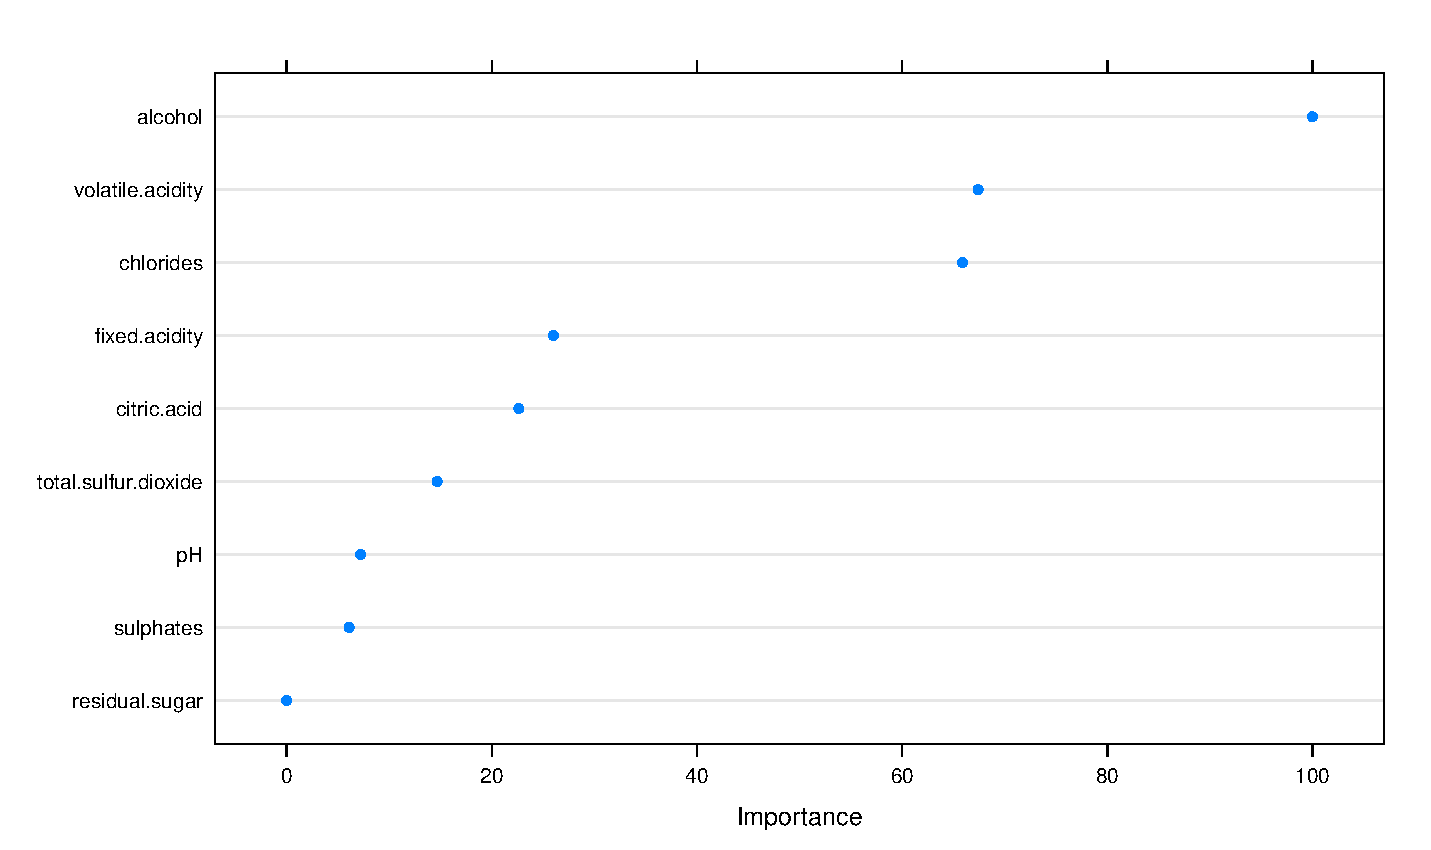
\includegraphics[scale=.25]{images/knnvarimp}}
\begin{knitrout}\footnotesize
\definecolor{shadecolor}{rgb}{0.969, 0.969, 0.969}\color{fgcolor}\begin{kframe}
\begin{alltt}
\hlkwd{dotPlot}\hlstd{(}\hlkwd{varImp}\hlstd{(results_knn))}
\end{alltt}
\end{kframe}
\end{knitrout}


\subsection{Strengths \& Weaknesses}
\emph{Strengths}\sidenote{See table 10.1 in \citet{hastie_elements_2009} for a more comprehensive list for this and the other methods discussed in this section.}
\begin{itemize}
  \item Intuitive approach.
  \item Robust to outliers on the predictors.
\end{itemize}


\noindent\emph{Weaknesses}
\begin{itemize}
  \item Susceptible to irrelevant features.
  \item Susceptible to correlated inputs.
  \item Ability to handle data of mixed types.
  \item Big data. Though approaches are available that help in this regard.
\end{itemize}

%%%
\section{Neural Nets}
\marginnote{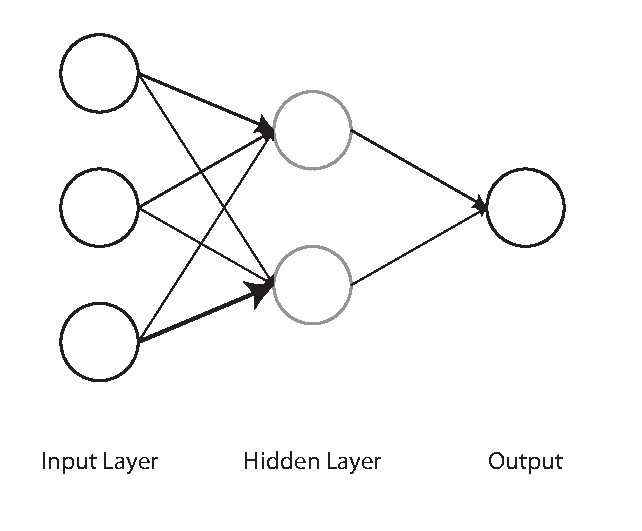
\includegraphics[scale=.5]{images/neural_net}}
Neural nets have been around for a long while as a general concept in artificial intelligence and even as a machine learning algorithm, and often work quite well.  In some sense they can be thought of as nonlinear regression.  Visually however, we can see them as layers of inputs and outputs.  Weighted combinations of the inputs are created and put through some function (e.g. the sigmoid function) to produce the next layer of inputs. This next layer goes through the same process to produce either another layer or to predict the output, which is the final layer\sidenote{There can be many output variables in this approach.}.  All the layers between the input and output are usually referred to as 'hidden' layers. If there were no hidden layers then it becomes the standard regression problem.

One of the issues with neural nets is determining how many hidden layers and how many hidden units in a layer.  Overly complex neural nets will suffer from high variance will thus be less generalizable, particularly if there is less relevant information in the training data.  Along with the complexity is the notion of \emph{weight decay}, however this is the same as the regularization function we discussed in a previous section, where a penalty term would be applied to a norm of the weights.

A comment about the following: if you are not set up for utilizing multiple processors the following might be relatively slow.  You can replace the method with $"nnet"$ and shorten the tuneLength to 3 which will be faster without much loss of accuracy.  Also, the function we're using has only one hidden layer, but the other neural net methods accessible via the caret package may allow for more, though the gains in prediction with additional layers are likely to be modest relative to complexity and computational cost. In addition, if the underlying function\sidenote{For this example, ultimately the primary function is \texttt{\textcolor{red}{nnet}} in the \emph{\textcolor{blue}{nnet}} package} has additional arguments, you may pass those on in the train function itself.  Here I am increasing the 'maxit', or maximum iterations, argument.

\begin{knitrout}\footnotesize
\definecolor{shadecolor}{rgb}{0.969, 0.969, 0.969}\color{fgcolor}\begin{kframe}
\begin{alltt}
\hlstd{results_nnet} \hlkwb{=} \hlkwd{train}\hlstd{(good}\hlopt{~}\hlstd{.,} \hlkwc{data}\hlstd{=wine_train,} \hlkwc{method}\hlstd{=}\hlstr{"avNNet"}\hlstd{,}
                     \hlkwc{trControl}\hlstd{=cv_opts,} \hlkwc{preProcess}\hlstd{=}\hlstr{"range"}\hlstd{,}
                     \hlkwc{tuneLength}\hlstd{=}\hlnum{5}\hlstd{,} \hlkwc{trace}\hlstd{=F,} \hlkwc{maxit}\hlstd{=}\hlnum{1000}\hlstd{)}
\hlstd{results_nnet}
\end{alltt}
\begin{verbatim}
## Model Averaged Neural Network 
## 
## 5199 samples
##    9 predictors
##    2 classes: 'Bad', 'Good' 
## 
## Pre-processing: re-scaling to [0, 1] 
## Resampling: Cross-Validated (10 fold) 
## 
## Summary of sample sizes: 4679, 4679, 4680, 4679, 4679, 4679, ... 
## 
## Resampling results across tuning parameters:
## 
##   size  decay  Accuracy  Kappa  Accuracy SD  Kappa SD
##   1     0      0.7       0.4    0.02         0.04    
##   1     1e-04  0.7       0.4    0.02         0.04    
##   1     0.001  0.7       0.4    0.02         0.04    
##   1     0.01   0.7       0.4    0.02         0.04    
##   1     0.1    0.7       0.4    0.02         0.04    
##   3     0      0.8       0.5    0.02         0.04    
##   3     1e-04  0.8       0.5    0.02         0.04    
##   3     0.001  0.8       0.5    0.02         0.04    
##   3     0.01   0.8       0.5    0.01         0.03    
##   3     0.1    0.8       0.5    0.01         0.03    
##   5     0      0.8       0.5    0.02         0.05    
##   5     1e-04  0.8       0.5    0.01         0.03    
##   5     0.001  0.8       0.5    0.02         0.04    
##   5     0.01   0.8       0.5    0.02         0.04    
##   5     0.1    0.8       0.5    0.01         0.03    
##   7     0      0.8       0.5    0.02         0.04    
##   7     1e-04  0.8       0.5    0.02         0.04    
##   7     0.001  0.8       0.5    0.01         0.03    
##   7     0.01   0.8       0.5    0.01         0.03    
##   7     0.1    0.8       0.5    0.01         0.03    
##   9     0      0.8       0.5    0.02         0.05    
##   9     1e-04  0.8       0.5    0.01         0.03    
##   9     0.001  0.8       0.5    0.01         0.03    
##   9     0.01   0.8       0.5    0.01         0.03    
##   9     0.1    0.8       0.5    0.01         0.03    
## 
## Tuning parameter 'bag' was held constant at a value of FALSE
## Accuracy was used to select the optimal model using  the largest value.
## The final values used for the model were size = 9, decay = 0 and bag
##  = FALSE.
\end{verbatim}
\end{kframe}
\end{knitrout}


We see that the best model has  hidden layer nodes and a decay parameter of .  Typically you might think of how many hidden units you want to examine in terms of the amount of data you have (i.e. estimated parameters to N ratio), and here we have a decent amount.  In this situation you might start with very broad values for the number of inputs (e.g. a sequence by 10s) and then narrow your focus (e.g. between 20 and 30), but with at least some weight decay you should be able to avoid overfitting. I was able to get an increase in test accuracy of about 1.5\% using up to 50 hidden units\sidenote{There are some rules of thumb, but using regularization and cross-validation is a much better way to 'guess'.}.

\begin{knitrout}\footnotesize
\definecolor{shadecolor}{rgb}{0.969, 0.969, 0.969}\color{fgcolor}\begin{kframe}
\begin{alltt}
\hlstd{preds_nnet} \hlkwb{=} \hlkwd{predict}\hlstd{(results_nnet, wine_test[,}\hlopt{-}\hlnum{10}\hlstd{])}
\hlkwd{confusionMatrix}\hlstd{(preds_nnet, wine_test[,}\hlnum{10}\hlstd{],} \hlkwc{positive}\hlstd{=}\hlstr{'Good'}\hlstd{)}
\end{alltt}


{\ttfamily\noindent\bfseries\color{errorcolor}{\#\# Error: could not find function "{}confusionMatrix"{}}}

{\ttfamily\noindent\bfseries\color{errorcolor}{\#\# Error: could not find function "{}confusionMatrix"{}}}\end{kframe}
\end{knitrout}


We note improved prediction with the neural net model relative to the k-nearest neighbors approach, with increases in accuracy (

{\ttfamily\noindent\bfseries\color{errorcolor}{\\Error in eval(expr, envir, enclos) : object 'conf\_nnet' not found}}\%), sensitivity, specificity etc.

\subsection{Strengths \& Weaknesses}

\emph{Strengths}
\begin{itemize}
  \item Good prediction generally.
  \item Incorporating the predictive power of different combinations of inputs.
  \item Some tolerance to correlated inputs.
\end{itemize}


\noindent\emph{Weaknesses}
\begin{itemize}
  \item Susceptible to irrelevant features.
  \item Not robust to outliers.
  \item Big data with complex models.
\end{itemize}

%%%
\section{Trees \& Forests}

Classification and regression trees provide yet another and notably different approach to prediction.  Consider a single input variable and binary dependent variable.  We will search all values of the input to find a point where, if we partition the data at that point, it will lead to the best classification accuracy.  \marginnote{\center{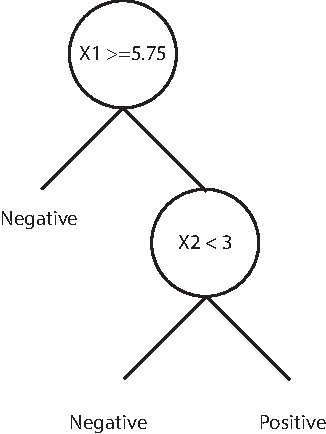
\includegraphics[scale=.5]{images/hypotree}}}So for a single variable whose range might be 1 to 10, we find that a cut at 5.75 results in the best classification if all observations greater than or equal to 5.75 are classified as positive and the rest negative.  This general approach is fairly straightforward and conceptually easy to grasp, and it is because of this that tree approaches are appealing.  


Now let's add a second input, also on a 1 to 10 range.  We now might find that even better classification results if, upon looking at the portion of data regarding those greater than or equal to 5.75, that we only classify positive if they are also less than 3 on the second variable.  At right is a hypothetical tree reflecting this.

\marginnote{\center{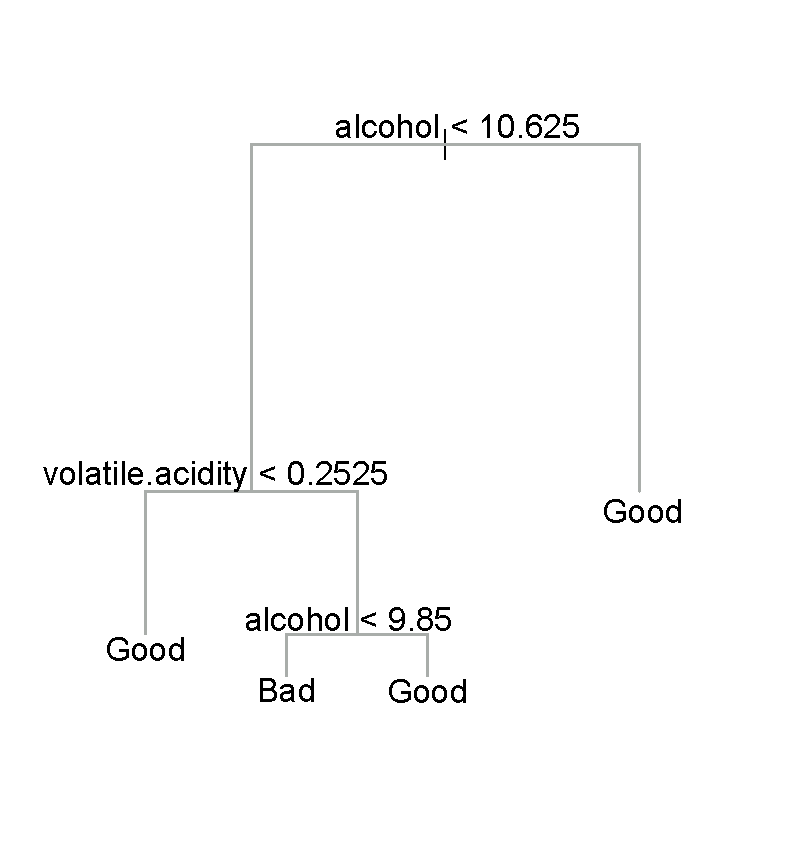
\includegraphics[scale=.5]{images/winetree}}\\
Results from the \textcolor{blue}{tree} package.}
The example tree here is based on the wine training data set. It is interpreted as follows.  If the alcohol content is greater than 10.63 \%, a wine is classified as good\sidenote{Color me unsurprised by this finding.}. For those less than 10.63, if its volatile acidity is also less than .25, they are also classified as good, and of the remaining observations, if they are at least more than 9.85\% (i.e. volatility >.25, alcohol between 9.85 and 10.625), they also get classified as good.  Any remaining observations are classified as bad wines.

Unfortunately a single tree, while highly interpretable, does pretty poorly for predictive purposes.  In standard situations we will instead use the power of many trees, i.e. a forest, based on repeated sampling of the original data.  So if we create 1000 new training data sets based on random samples of the original data (each of size N, i.e. a bootstrap of the original data set), we can run a tree for each, and assess the predictions each tree would produce for the observations for a hold out set (or simply those observations which weren't selected during the sampling process, the 'out-of-bag' sample), in which the new data is 'run down the tree' to obtain predictions. The final class prediction for an observation is determined by majority vote across all trees.

Random forests are referred to as an \emph{ensemble} method, one that is actually a combination of many models, and there are others we'll mention later.  In addition there are other things to consider, such as how many variables to make available for consideration at each split, and this is the tuning parameter of consequence here in our use of caret (called 'mtry').  In this case we will investigate subsets of 2 through 6 possible predictors. With this value determined via cross-validation, we can apply the best approach to the hold out test data set.

There's a lot going on here to be sure: there is a sampling process for cross-validation, there is resampling to produce the forest, there is random selection of mtry predictor variables etc.  But we are in the end just harnessing the power of many trees, any one of which would be highly interpretable.

%For all 9-1 splits of the data,
%Create 1000 random resamples of size $N_9$,
%For each t of 1000, create a tree
%At each split of each tree, randomly pick mtry predictor variables as potential splitter variables.
%Examine performance on the kth partition of data.
%Select the mtry that produces the best performance.
%Run the test data through the selected forest.

\begin{knitrout}\footnotesize
\definecolor{shadecolor}{rgb}{0.969, 0.969, 0.969}\color{fgcolor}\begin{kframe}
\begin{alltt}
\hlkwd{set.seed}\hlstd{(}\hlnum{1234}\hlstd{)}
\hlstd{rf_opts} \hlkwb{=} \hlkwd{data.frame}\hlstd{(}\hlkwc{.mtry}\hlstd{=}\hlkwd{c}\hlstd{(}\hlnum{2}\hlopt{:}\hlnum{6}\hlstd{))}
\hlstd{results_rf} \hlkwb{=} \hlkwd{train}\hlstd{(good}\hlopt{~}\hlstd{.,} \hlkwc{data}\hlstd{=wine_train,} \hlkwc{method}\hlstd{=}\hlstr{"rf"}\hlstd{,}
                   \hlkwc{preProcess}\hlstd{=}\hlstr{'range'}\hlstd{,}\hlkwc{trControl}\hlstd{=cv_opts,} \hlkwc{tuneGrid}\hlstd{=rf_opts,}
                   \hlkwc{n.tree}\hlstd{=}\hlnum{1000}\hlstd{)}
\hlstd{results_rf}
\end{alltt}
\begin{verbatim}
## Random Forest 
## 
## 5199 samples
##    9 predictors
##    2 classes: 'Bad', 'Good' 
## 
## Pre-processing: re-scaling to [0, 1] 
## Resampling: Cross-Validated (10 fold) 
## 
## Summary of sample sizes: 4679, 4679, 4680, 4679, 4679, 4679, ... 
## 
## Resampling results across tuning parameters:
## 
##   mtry  Accuracy  Kappa  Accuracy SD  Kappa SD
##   2     0.8       0.6    0.02         0.04    
##   3     0.8       0.6    0.02         0.04    
##   4     0.8       0.6    0.02         0.04    
##   5     0.8       0.6    0.02         0.04    
##   6     0.8       0.6    0.02         0.03    
## 
## Accuracy was used to select the optimal model using  the largest value.
## The final value used for the model was mtry = 2.
\end{verbatim}
\end{kframe}
\end{knitrout}


The initial results look promising with mtry =  producing the best initial result.  Now for application to the test set.

\begin{knitrout}\footnotesize
\definecolor{shadecolor}{rgb}{0.969, 0.969, 0.969}\color{fgcolor}\begin{kframe}
\begin{alltt}
\hlstd{preds_rf} \hlkwb{=} \hlkwd{predict}\hlstd{(results_rf, wine_test[,}\hlopt{-}\hlnum{10}\hlstd{])}
\hlkwd{confusionMatrix}\hlstd{(preds_rf, wine_test[,}\hlnum{10}\hlstd{],} \hlkwc{positive}\hlstd{=}\hlstr{'Good'}\hlstd{)}
\end{alltt}
\begin{verbatim}
## Confusion Matrix and Statistics
## 
##           Reference
## Prediction Bad Good
##       Bad  335   91
##       Good 141  731
##                                         
##                Accuracy : 0.821         
##                  95% CI : (0.799, 0.842)
##     No Information Rate : 0.633         
##     P-Value [Acc > NIR] : <2e-16        
##                                         
##                   Kappa : 0.606         
##  Mcnemar's Test P-Value : 0.0013        
##                                         
##             Sensitivity : 0.889         
##             Specificity : 0.704         
##          Pos Pred Value : 0.838         
##          Neg Pred Value : 0.786         
##              Prevalence : 0.633         
##          Detection Rate : 0.563         
##    Detection Prevalence : 0.672         
##       Balanced Accuracy : 0.797         
##                                         
##        'Positive' Class : Good          
## 
\end{verbatim}
\end{kframe}
\end{knitrout}


This is our best result so far with 82.13\% accuracy, with a lower bound well beyond the 63\% we'd have guessing.  Random forests do not suffer from some of the data specific issues that might be influencing the other approaches, such as irrelevant and correlated predictors, and furthermore benefit from the combined information of many models.  Such performance increases are not a given, but random forests are generally a good method to consider given their flexibility.

Incidentally, the underlying \textcolor{red}{randomForest} function here allows one to assess variable importance in a different manner\sidenote{Our previous assessment was model independent.}, and there are other functions used by caret that can produce their own metrics also.  In this case, randomForest can provide importance based on a version of the 'decrease in inaccuracy' approach we talked before (as well as another index known as gini impurity).  The same two predictors are found to be most important and notably more than others- alcohol and volatile.acidity.

\subsection{Strengths \& Weaknesses}

\emph{Strengths}
\begin{itemize}
  \item A single tree is highly interpretable.
  \item Tolerance to irrelevant features.
  \item Some tolerance to correlated inputs.
  \item Good with big data.
  \item Handling of missing values.
\end{itemize}

\marginnote{\raggedleft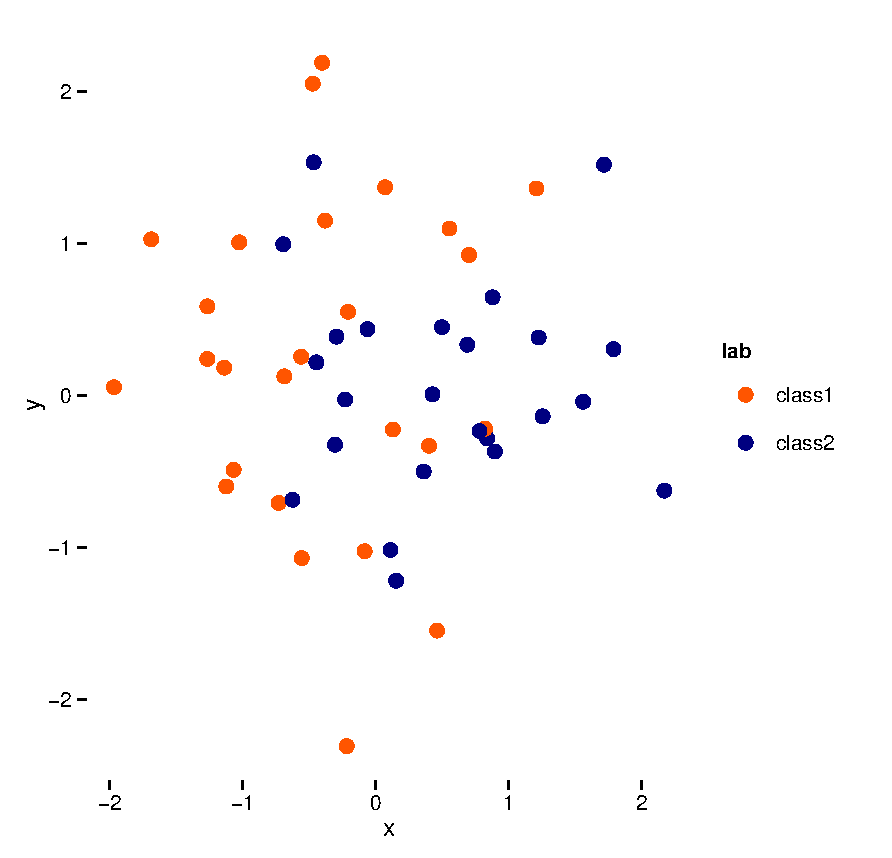
\includegraphics[scale=.35]{images/svm2d}\\
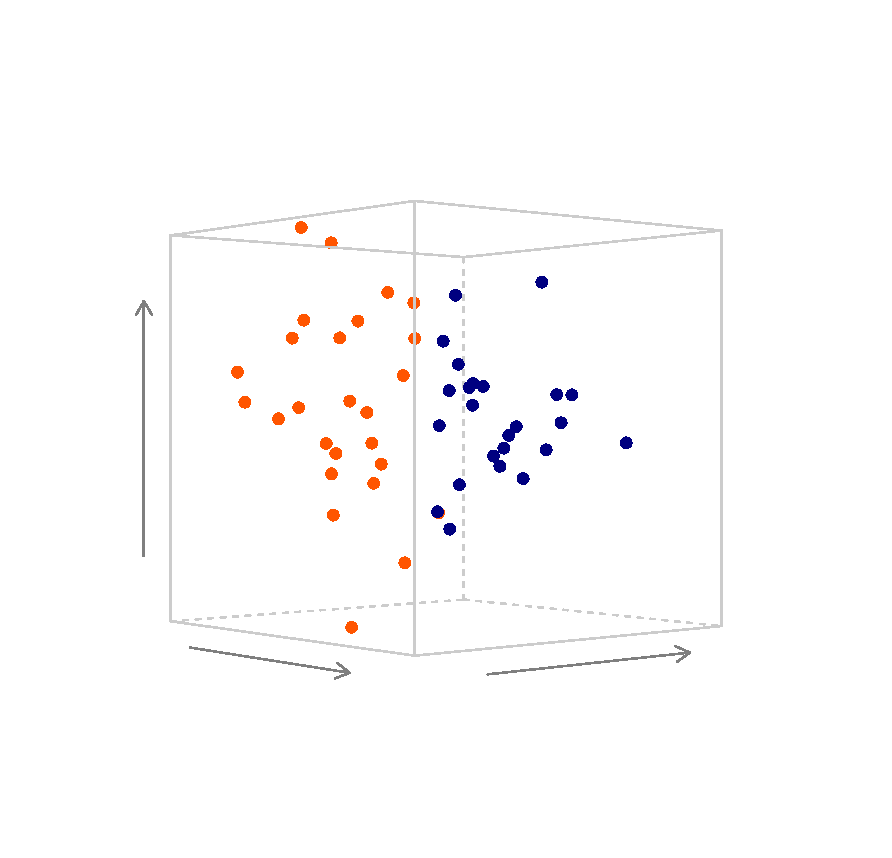
\includegraphics[scale=.35]{images/svm3d}\\
}


\noindent\emph{Weaknesses}
\begin{itemize}
  \item Relatively less predictive in many situations.
  \item Cannot work on (linear) combinations of features.
\end{itemize}

%%%

\section{Support Vector Machines}

Support Vector Machines (SVM) will be our last example, and is perhaps the least intuitive.  SVMs seek to map the input space to a higher dimension via a kernel function, and in that transformed feature space, find a hyperplane that will result in maximal separation of the data.   

To better understand this process, consider the example to the right of two inputs, $x$ and $y$. Cursory inspection shows no easy separation between classes.  However if we can map the data to a higher dimension\sidenote{Note that we regularly do this sort of thing in more mundane circumstances.  For example, we map an $Nxp$ matrix to an $NxN$ matrix when we compute a distance matrix for cluster analysis.}, shown in the following graph, we might find a more clear separation. Note that there are a number of choices in regard to the kernel function that does the mapping, but in that higher dimension, the decision boundary is chosen which will result in maximum distance (largest margin) between classes (following figures, zoom in to see the margin on the second plot).  Real data will not be so clean cut, and total separation impossible, but the idea is the same.
\marginnote{\raggedleft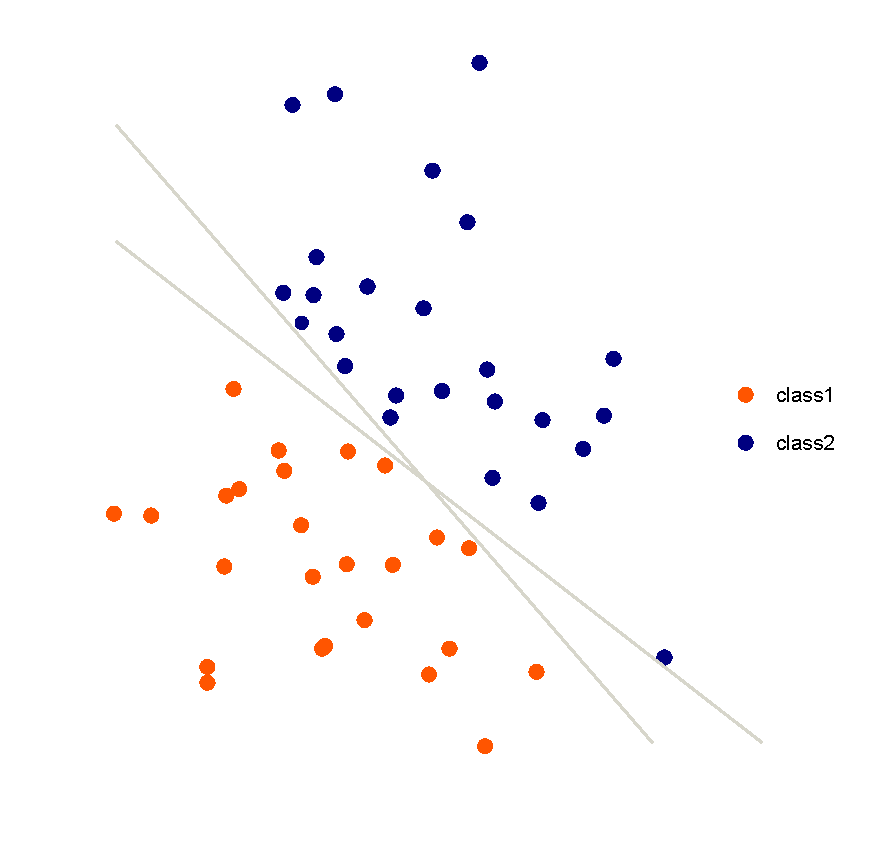
\includegraphics[scale=.30]{images/svmSeparate1}\\
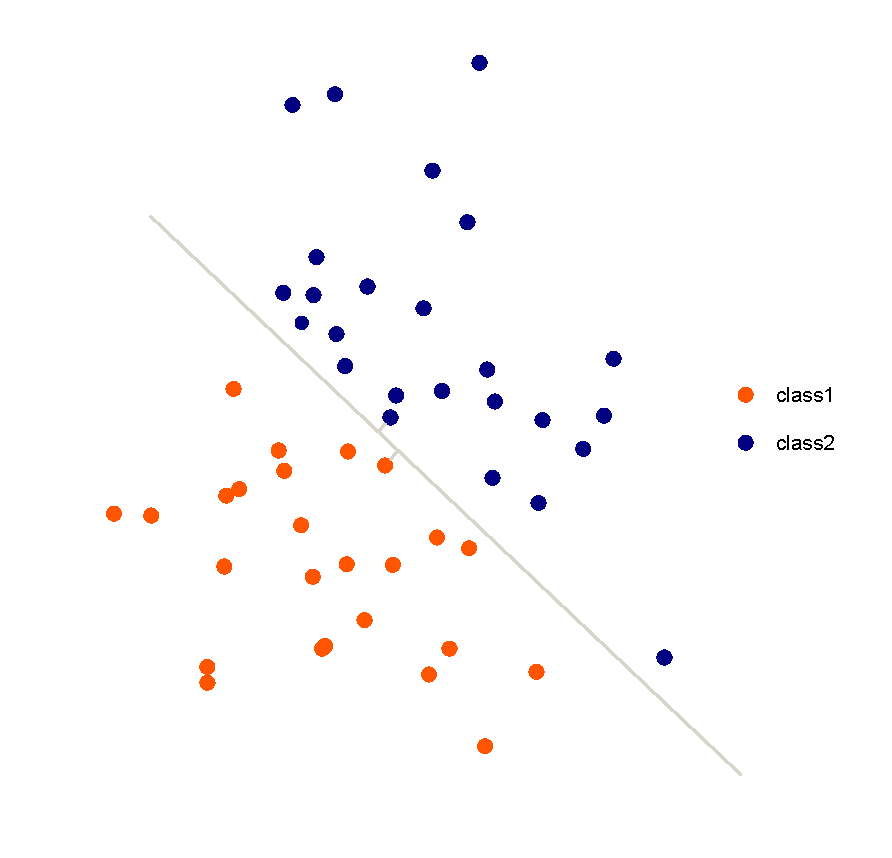
\includegraphics[scale=.30]{images/svmSeparate2}
}

\begin{knitrout}\footnotesize
\definecolor{shadecolor}{rgb}{0.969, 0.969, 0.969}\color{fgcolor}\begin{kframe}
\begin{alltt}
\hlkwd{set.seed}\hlstd{(}\hlnum{1234}\hlstd{)}
\hlstd{results_svm} \hlkwb{=} \hlkwd{train}\hlstd{(good}\hlopt{~}\hlstd{.,} \hlkwc{data}\hlstd{=wine_train,} \hlkwc{method}\hlstd{=}\hlstr{"svmLinear"}\hlstd{,}
                    \hlkwc{preProcess}\hlstd{=}\hlstr{"range"}\hlstd{,} \hlkwc{trControl}\hlstd{=cv_opts,} \hlkwc{tuneLength}\hlstd{=}\hlnum{5}\hlstd{)}
\hlstd{results_svm}
\end{alltt}
\begin{verbatim}
## Support Vector Machines with Linear Kernel 
## 
## 5199 samples
##    9 predictors
##    2 classes: 'Bad', 'Good' 
## 
## Pre-processing: re-scaling to [0, 1] 
## Resampling: Cross-Validated (10 fold) 
## 
## Summary of sample sizes: 4679, 4679, 4680, 4679, 4679, 4679, ... 
## 
## Resampling results
## 
##   Accuracy  Kappa  Accuracy SD  Kappa SD
##   0.7       0.4    0.02         0.05    
## 
## Tuning parameter 'C' was held constant at a value of 1
## 
\end{verbatim}
\end{kframe}
\end{knitrout}


\begin{knitrout}\footnotesize
\definecolor{shadecolor}{rgb}{0.969, 0.969, 0.969}\color{fgcolor}\begin{kframe}
\begin{alltt}
\hlstd{preds_svm} \hlkwb{=} \hlkwd{predict}\hlstd{(results_svm, wine_test[,}\hlopt{-}\hlnum{10}\hlstd{])}
\hlkwd{confusionMatrix}\hlstd{(preds_svm, wine_test[,}\hlnum{10}\hlstd{],} \hlkwc{positive}\hlstd{=}\hlstr{'Good'}\hlstd{)}
\end{alltt}
\begin{verbatim}
## Confusion Matrix and Statistics
## 
##           Reference
## Prediction Bad Good
##       Bad  269  123
##       Good 207  699
##                                         
##                Accuracy : 0.746         
##                  95% CI : (0.721, 0.769)
##     No Information Rate : 0.633         
##     P-Value [Acc > NIR] : < 2e-16       
##                                         
##                   Kappa : 0.432         
##  Mcnemar's Test P-Value : 4.9e-06       
##                                         
##             Sensitivity : 0.850         
##             Specificity : 0.565         
##          Pos Pred Value : 0.772         
##          Neg Pred Value : 0.686         
##              Prevalence : 0.633         
##          Detection Rate : 0.539         
##    Detection Prevalence : 0.698         
##       Balanced Accuracy : 0.708         
##                                         
##        'Positive' Class : Good          
## 
\end{verbatim}
\end{kframe}
\end{knitrout}


Results for the initial support vector machine do not match the random forest for this data set, with accuracy of 74.58\%.  However, you might choose a different kernel than the linear one used here, as well as tinker with other options.


\subsection{Strengths \& Weaknesses}

\emph{Strengths}
\begin{itemize}
  \item Good prediction in a variety of situations.
  \item Can utilize predictive power of linear combinations of inputs.
\end{itemize}


\noindent\emph{Weaknesses}
\begin{itemize}
  \item Very black box.
  \item Computational scalability.
  \item Natural handling of mixed data types.
\end{itemize}





% !Rnw root = ../mlcrash.Rnw




%%%%%%%%%%%%
\part{Other}
%%%%%%%%%%%%
\newthought{In this section I note some other techniques} one may come across and others that will provide additional insight into machine learning applications.

%%%
\section{Unsupervised Learning}
Unsupervised learning generally speaking involves techniques in which we are utilizing unlabeled data. In this case we have our typical set of features we are interested in, but no particular response to map them to.  In this situation we are more interested in the discovery of structure within the data.

\subsection{Clustering}
Many of the techniques used in unsupervised are commonly taught in various applied disciplines as various forms of "cluster" analysis.  The gist is we are seeking an unknown class structure rather than seeing how various inputs relate to a known class structure.  Common techniques include k-means, hierarchical clustering, and model based approaches (e.g. mixture models).

\subsection{Latent Variable Models}
\marginnote{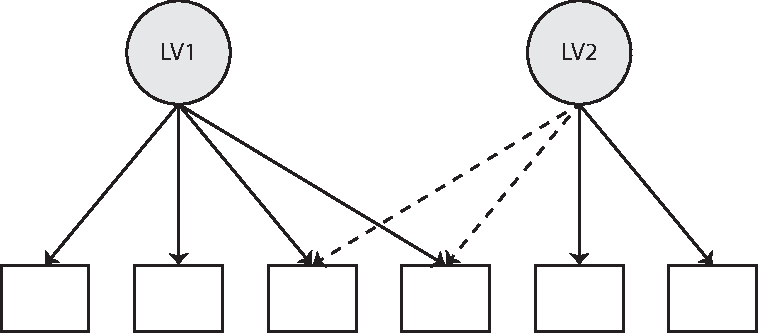
\includegraphics[scale=.35]{images/lvmodel}}
Sometimes the desire is to reduce the dimensionality of the inputs to a more manageable set of information.  In this manner we are thinking that much of the data can be seen as having only a few sources of variability, often called latent variables or factors.  Again, this takes familiar forms such as principal components and ("exploratory") factor analysis, but would also include independence components analysis and partial least squares techniques.  Note also that these can be part of a supervised technique (e.g. principal components regression) or the main focus of analysis (as with latent variable models in structural equation modeling).

\subsection{Graphical Structure}
\marginnote {\begin{center}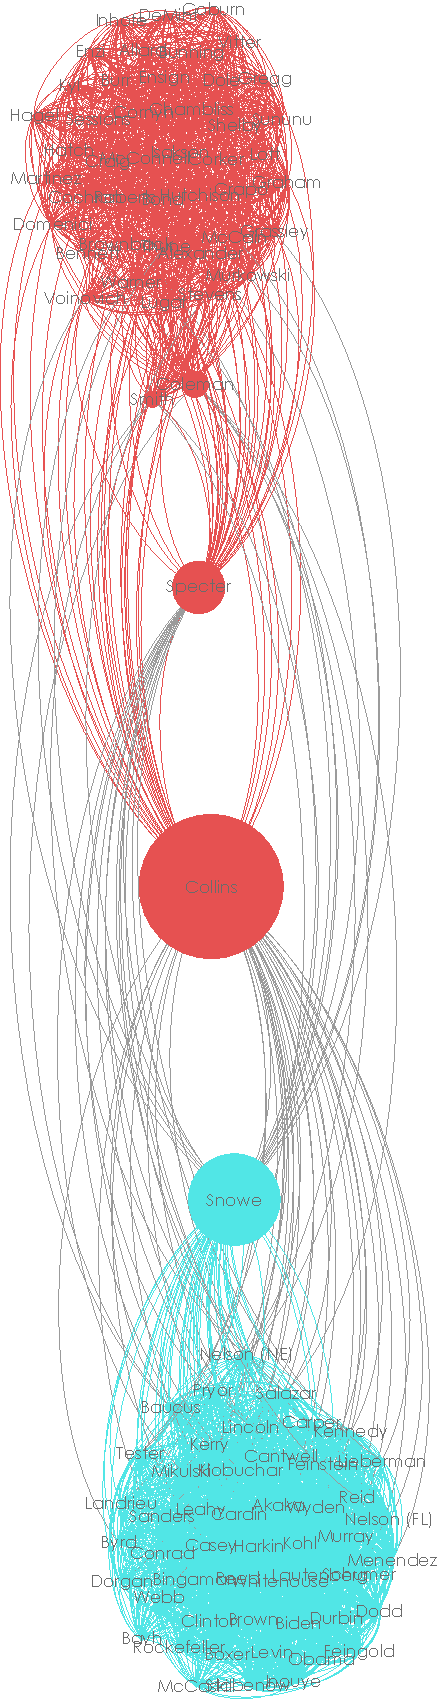
\includegraphics[scale=.35]{images/senategraph}\end{center} Example graph of the social network of senators based on data and filter at the following link. Node size is based on the \emph{betweeness} centrality measure, edge size the percent agreement (graph filtered to edges >= 65\%). Color is based on the clustering discovered within the graph. Zoom in as necessary, and note that you may need to turn off 'enhance thin lines' in your Adobe Page Display Preferences if using it as a viewer. \href{http://support.google.com/fusiontables/answer/2566732?hl=en&ref_topic=2572801}{link to data}.}
Other techniques are available to understand structure among observations or features.  Among the many approaches is the popular \emph{network analysis}, where we can obtain similarities among observations and examine visually the structure of those data points, where observations are placed closer together that are more similar in nature. In still other situations, we aren't so interested in the structure as we are in modeling the relationships and making predictions from the correlations of inputs.

\subsection{Imputation}
We can also use these techniques when we are missing data as a means to impute the missing values\sidenote{This and other techniques may fall under the broad heading of matrix completion.}.  While many are familiar with this problem and standard techniques for dealing with it, it may not be obvious that ML techniques may also be used.  For example, both k-nearest neighbors and random forest techniques have been applied to imputation. 

Beyond this we can infer values that are otherwise unavailable in a different sense.  Consider Netflix, Amazon and other sites that suggest various products based on what you already like or are interested in.  In this case the suggested products have missing values for the user which are imputed or inferred based on their available data and other consumers similar to them who have rated the product in question.  Such \emph{recommender systems} are widely used these days.

%%%
\section{Ensembles}
In many situations we can combine the information of multiple models to enhance prediction.  This can take place within a specific technique, e.g. random forests, or between models that utilize different techniques.  I will discuss some standard techniques, but there are a great variety of forms in which model combination might take place.

\subsection{Bagging}
\emph{Bagging}, or bootstrap aggregation, uses bootstrap sampling to create many data sets on which a procedure is then performed.  The final prediction is based on an average of all the predictions made for each observation.  In general, bagging helps reduce the variance while leaving bias unaffected. A conceptual outline of the procedure is provided.

\medskip
\noindent \emph{Model Generation} \\
For $B$ number of iterations:
\begin{enumerate}
  \item Sample $N$ observations with replacement $B$ times to create $B$ data sets of size $N$.
  \item Apply the learning technique to each of $B$ data sets to create $t$ models.
  \item Store the $t$ results.
\end{enumerate}
\emph{Classification} \\
For each of $t$ number of models:
\begin{enumerate}
  \item Predict the class of $N$ observations of the original data set.
  \item Return the class predicted most often.
\end{enumerate}

\subsection{Boosting}
With \emph{boosting} we take a different approach to refitting models.  Consider a classification task in which we start with a basic learner and apply it to the data of interest.  Next the learner is refit, but with more weight (importance) given to \emph{misclassified} observations.  This process is repeated until some stopping rule is reached.  An example of the AdaBoost algorithm is provided (in the following $\mathbb{I}$ is the indicator function).

\medskip
\small
\begin{itemize}
  \item Set initial weights $w_i$ to $1/N$.
  \item for $m=1:M$ \quad\{
    \item \qquad Fit a classifier $m$ with given weights to the data resulting in  \\ \qquad predictions $f^{(m)}_i$ that minimizes some loss function.
    \item \qquad Compute the error rate $err_m = \frac{\overset{N}{\underset{i=1}{\sum}} \mathbb{I}(y_i\ne f^{(m)}_i)}{\overset{N}{\underset{i=1}{\sum}}w^{(m)}_i}$
    \item \qquad Compute $\alpha_m = \log[(1-err_m)/err_m]$
    \item \qquad Set $w_i \leftarrow w_i\exp[\alpha_m \mathbb{I}(y_i\ne f^{(m)}_i)]$ \\
    \} \\
    \texttt{Return} $\sgn [\overset{M}{\underset{m=1}{\sum}}\alpha_m f^{(m)}]$
\end{itemize}
\normalsize

\medskip
Boosting can be applied to a variety of tasks and loss functions, and in general is highly resistant to overfitting.

\subsection{Stacking}
\emph{Stacking} is a method that can generalize beyond a single fitting technique, though it can be applied in a fashion similar to boosting for a single technique.  While the term can refer to a specific technique, here we will use it broadly to mean any method to combine models of different forms. Consider the four approaches we demonstrated earlier: k-nearest neighbors, neural net, random forest, and the support vector machine.  We saw that they do not have the same predictive accuracy, though they weren't bad in general. Perhaps by combining their respective efforts, we could get even better prediction than using any particular one. 

The issue then how we might combine them.  We really don't have to get too fancy with it, and can even use a simple voting scheme as in bagging. For each observation, note the predicted class on new data across models. The final prediction is the class that receives the most votes.  Another approach would be to use a weighted vote, where the votes are weighted by their respective accuracies.  

Another approach would use the predictions on the test set to create a data set of just the predicted probabilities from each learning scheme. We can then use this data to train a meta-learner using the test labels as the response.  With the final meta-learner chosen, we then retrain the original models on the entire data set (i.e. including the test data).  In this manner the initial models and the meta-learner are trained separately and you get to eventually use the entire data set to train the original models.  Now when new data becomes available, you feed them to the base level learners, get the predictions, and then feed the predictions to the meta-learner for the final prediction.

%%%
\section{Feature Selection \& Importance}
We hit on this topic some before, but much like there are a variety of ways to gauge performance, there are different approaches to select features and/or determine their importance. Invariably feature selection takes place from the outset when we choose what data to collect in the first place.  Hopefully guided by theory, in other cases it may be restricted by user input, privacy issues, time constraints and so forth.  But once we obtain the initial data set however, we may still want to trim the models under consideration.

In standard approaches we might have in the past used forward or other selection procedure, or perhaps some more explicit model comparison approach.  Concerning the content here, take for instance the lasso regularization procedure we spoke of earlier.  'Less important' variables may be shrunk entirely to zero, and thus feature selection is an inherent part of the process, and is useful in the face of many, many predictors, sometimes outnumbering our sample points. As another example, consider any particular approach where the importance metric might be something like the drop in accuracy when the variable is excluded.

Variable importance was given almost full weight in the discussion of typical applied research in the past, based on statistical significance results from a one-shot analysis, and virtually ignorant of prediction on new data.  We still have the ability to focus on feature performance with ML techniques, while shifting more of the focus toward prediction at the same time.  For the uninitiated, it might require new ways of thinking about how one measures importance though.

%%%
\section{Textual Analysis}
In some situations the data of interest is not in a typical matrix form but in the form of textual content, i.e. a corpus of documents (loosely defined).  In this case, much of the work (like in most analyses but perhaps even more so) will be in the data preparation, as text is rarely if ever in a ready-to-analyze state.  The eventual goals may include using the word usage in the prediction of an outcome, perhaps modeling the usage of select terms, or examining the structure of the term usage graphically as in a network model.  In addition, machine learning processes might be applied to sounds (acoustic data) to discern the speech characteristics and other information.

%%%
\section{Bayesian Approaches}
It should be noted that the approaches outlined in this document are couched in the frequentist tradition.  But one should be aware that many of the concepts and techniques would carry over into the Bayesian perspective, and even some machine learning techniques might only be feasible or make more sense within the Bayesian framework (e.g. online learning). 


%%%
\section{More Stuff}
Aside from what has already been noted, there still exists a great many applications for ML such as data set shift
\sidenote{Used when fundamental changes occur between the data a learner is trained on and the data coming in for further analysis.}, 
deep learning\sidenote{Learning at different levels of representation, e.g. from an image regarding a scene to the concepts used to describe it.}, 
semi-supervised learning\sidenote{Learning with both labeled and unlabeled data.}, 
online learning\sidenote{Learning from a continuous stream of data.}, and many more.  









% !Rnw root = ../mlcrash.Rnw





%%%%%%%%%%%%%%
\part{Summary}
%%%%%%%%%%%%%%
\section{Cautionary Notes}
A standard mantra in machine learning and statistics generally is that there is no free lunch.  All methods have certain assumptions, and if those don't hold the results will be problematic at best.  Also, even if in truth learner A is better than B, B can often outperform A in the finite situations we actually deal with in practice.  Furthermore, being more complicated doesn't mean a technique is better.  As previously noted, incorporating regularization and cross-validation goes a long way toward to improving standard techniques, and they may perform quite well in some situations.

\section{Some Guidelines}
Here are some thoughts to keep in mind, though these may be applicable to applied statistical practice generally.
\medskip

\noindent More data beats a cleverer algorithm, but a lot of data is not enough by itself\sidenote{\citet{domingos_few_2012}}. 

\smallskip
\noindent Avoid overfitting.

\smallskip
\noindent Let the data speak for itself. 

\smallskip
\noindent "Nothing is more practical than a good theory."\sidenote{Kurt Lewin, and iterated by V. Vapnik for the machine learning context.}

\smallskip
\noindent While getting used to ML, it might be best to start from simpler approaches and then work towards more black box ones that require more tuning. For example, naive Bayes $\rightarrow$ logistic regression $\rightarrow$ knn $\rightarrow$ svm.

\smallskip
\noindent Drawing up a visual path of your process is a good way to keep your analysis on the path to your goal.  Some programs can even make this explicit (e.g. RapidMiner, Weka).

\smallskip
\noindent Keep the tuning parameter/feature selection process separate from the final test process for assessing error.

\smallskip
\noindent Learn multiple models, selecting the best or possibly combining them.

\section{Conclusion}
It is hoped that this document sheds some light on some areas that might otherwise be unfamiliar to some applied researchers. The field of statistics has rapidly evolved over the past two decades.  The tools available are myriad, and expanding all the time.  Rather than being overwhelmed, one should embrace the choice available, and have some fun with your data.






\pagebreak

% !Rnw root = mlcrash.Rnw




\part{Brief Glossary of Common Terms}
\begin{description}
  \item[bias] could mean the intercept (e.g. in neural nets), typically refers to the bias in bias-variance decomposition
  \item[regularization, penalization, shrinkage] The process of adding a penalty to the size of coefficients, thus shrinking them towards zero but resulting in less overfitting (at an increase to bias)
  \item[classifier] specific model or technique (i.e. function) that maps observations to classes
  \item[confusion matrix] a table of predicted class membership vs. true class membership
  \item[hypothesis] a specific model $h(x)$ of all possible in the hypothesis space $\mathcal{H}$
  \item[input, feature, attribute] independent variable, predictor variable, column
  \item[instance, example] observation, row
  \item[learning] model fitting
  \item[machine learning] a form of statistics utilizing various algorithms with a goal to generalize to new data situations
  \item[supervised] has a dependent variable
  \item[target, label] dependent variable, response, the outcome of interest
  \item[unsupervised] no dependent variable; think clustering, PCA etc.
  \item[weights]  coefficients, parameters
\end{description}









\pagebreak



\bibliography{MLtechrep}
I had a lot of sources in putting this together, but I note these in particular as I feel they can either provide the appropriate context to begin, help with the transition from more standard approaches, or serve as a definitive reference for various methods.

%\nocite{banko_scaling_2001}  % remove page numbers from bib file
%\nocite{tibshirani_regression_1996}
\nocite{breiman_statistical_2001}
\nocite{wood_generalized_2006}
\nocite{hastie_elements_2009}
\nocite{harrell_regression_2001}
\nocite{domingos_few_2012} % remove page numbers from bib file
\nocite{murphy_machine_2012}



\end{document}
